\documentclass[margin=5in, 12pt]{article}

\usepackage[utf8]{inputenc}
\usepackage[affil-it]{authblk}
\usepackage[margin=1in]{geometry}
\usepackage{multirow}
\usepackage{natbib}
\usepackage{graphicx}
\usepackage{float}
\graphicspath{{figures/}{./}}
\usepackage{amsmath}
\usepackage{amssymb}
\usepackage{amsfonts}
\usepackage{amstext}
\usepackage{bbm}
\usepackage{subcaption}
\usepackage[dvipsnames]{xcolor}
\usepackage{newpxtext,newpxmath}
\usepackage{url}
\usepackage{bm}
\setlength{\parskip}{.75em}
\geometry{margin=1in}
\let\openbox\relax % avoid clash between newpxmath and amsthm
\usepackage{amsthm}
\newtheorem{assumption}{Assumption}
\newtheorem{remark}{Remark}
\newtheorem{definition}{Definition}
\newtheorem{lemma}{Lemma}
\newtheorem{proposition}{Proposition}
\usepackage{booktabs}
\DeclareMathOperator{\RSS}{RSS}
\DeclareMathOperator{\E}{\mathbb{E}}
\DeclareMathOperator{\Var}{Var}
\newcommand{\DP}{\mathrm{DP}}
\newcommand{\Normal}{\mathcal{N}}
\newcommand{\R}{\mathbb{R}}
\newcommand{\1}{\mathbbm{1}}
\newcommand{\ytd}{\tilde{y}}
\newcommand{\Dtd}{\tilde{D}}
\newcommand{\Xtd}{\tilde{X}}

\title{\textbf{Specification in TWFE in Staggered
       Timing and Partial Heterogeneous Effect}%
       }
\author{Parush Arora$^*$ and Rohan Wagle\thanks{Department of Economics, Ashoka University.}}
\date{}

\begin{document}
\maketitle

% =============================================================================
% ABSTRACT
% =============================================================================
\begin{abstract}
  \noindent
  In staggered difference-in-differences (DiD) designs, units enter treatment at
  different calendar times, so the treatment effect is not a single number but a
  set of Cohort-Average Treatment effects on the Treated (CATTs), one per
  cohort-time cell. Estimating every CATT as its own parameter, as the standard
  fully flexible estimator does, is unbiased but inefficient when some of these
  effects are in fact equal, whereas pooling them all into a single two-way fixed effects
  (TWFE) coefficient is efficient but biased whenever the heterogeneity is genuine.
  We frame the choice between these extremes as a partition-selection
  problem on the cohort-time cells and address it with a Dirichlet
  Process (DP) mixture prior on the CATTs. The model favors parsimonious groupings
  without fixing their number, and a collapsed Gibbs sampler delivers point
  estimates, credible intervals that marginalize the unknown partition, and
  co-clustering probabilities for every pair of CATTs. As an aside, with the
  error variance held fixed the model's maximum a posteriori (MAP) partition
  reduces to an $\ell_0$-penalized regression, connecting the Bayesian
  formulation to the homogeneity-pursuit literature.
  In a calibrated simulation, the model cuts the sampling variance of the
  cohort-time effects by 26--52\% relative to the fully flexible estimator, without
  the pooled estimator's bias, provided the distinct effects are separated enough
  to be recovered, and the posterior delivers near-nominal confidence-interval
  coverage by averaging over the unknown partition.
  In two applications the method recovers a precision-improving
  partial-homogeneity structure in one, where the cohort-time effects are
  genuinely heterogeneous, and reports that full pooling is adequate in the
  other, where they are not.
\end{abstract}

\bigskip
\noindent\textbf{Keywords:} difference-in-differences, staggered treatment, TWFE, model specification, Bayesian estimation, Gibbs sampler,
treatment effect heterogeneity, causal inference.

\bigskip
\noindent\textbf{JEL Codes:} C11, C14, C23, C52.

\newpage

% =============================================================================
% 1. INTRODUCTION
% =============================================================================
\section{Introduction}
\label{sec:intro}

Difference-in-differences (DiD) has become one of the workhorses of empirical economics. In its canonical form, a treatment cohort and a control cohort are observed before and after a single policy change, and the researcher estimates a single average treatment effect (ATT or average treatment effect on treated). In a simple setting with two time periods, ATT is recovered by taking the difference between the change in the average outcome over time for the treatment and control cohorts, commonly referred to as a simple $2\times2$ DiD estimate. In a general setting with $N$ observations and $T$ time periods, the most popular way to estimate the ATT with a binary treatment indicator is the two-way fixed effects regression (TWFE):
\begin{equation}
\label{eq:rest_twfe}
  Y_{it} = \alpha_i + \lambda_t + \tau D_{it} + \varepsilon_{it},
\end{equation}
where $Y_{it}$ is the observed outcome for $i^{th}$ unit in time $t$, $\alpha_i$ is the unit fixed effect, $\lambda_t$ is the time fixed effect, $D_{it}$ is the treatment dummy and $\tau$ is the ATT. We will refer to Eq.~\ref{eq:rest_twfe} as pooled TWFE. The pooled TWFE estimator ($\hat\tau_{\text{pool}}$) is directly related to the $2\times 2$ DiD estimator, as it can be represented as a weighted average of all possible 2$\times$2 DiD estimates \citep{goodman2021}.


Modern policy evaluations, however, rarely fit this clean template. Minimum wage increases, Medicaid expansions, trade liberalizations, and school reforms typically roll out across states, cities, or firms in a staggered fashion, with different units adopting treatment at different calendar times. We update the notation so that $Y_{igt}$ and $D_{igt}$ denote the outcome and treatment indicator for unit $i$ in cohort $g$ at time $t$. The estimator $\hat\tau_{\text{pool}}$ is unbiased in staggered timing if the treatment effect for each $g\times t$ case (cohort-time specific ATT or CATT) is homogeneous.

The econometrics of staggered DiD has seen remarkable progress in recent years. \citet{dechaisemartin2020}, \citet{callaway2021}, \citet{sun2021}, \citet{goodman2021}, \citet{gardner2022two}, and
\citet{borusyak2024}, among others, have shown that the TWFE regression can produce a biased estimate of the ATT when there is heterogeneity among CATTs. \citet{dechaisemartin2023} and \citet{roth2023} survey this literature. The bias arises due to the inclusion of an already-treated cohort as a control, which violates the parallel trends assumption. \citet{goodman2021} showed that the decomposition of TWFE can contain negative weights when the treatment effects are heterogeneous. The recommended solution is to either drop the already-treated cohorts from the control or estimate the CATTs one coefficient per (cohort-time) cell and then aggregate them as desired. For the latter, \citet{wooldridge2025} discussed the flexible TWFE that allows interaction between the treatment dummy and the cohort-time dummy and recovers unbiased CATTs. Their estimate is identical to \citet{gardner2022two} and \citet{borusyak2024} in certain settings and more efficient than \citet{callaway2021} and \citet{sun2021}, which drop the already-treated cohorts from the control. These heterogeneity-robust estimators are efficient only under spherical errors. \citet{arora2026} show that efficiency under arbitrary within-unit serial correlation is attainable through an optimally weighted GMM in the space of clean comparisons.

This fully flexible approach solves the bias problem but introduces a new challenge, namely model specification. With $G$ treated cohorts and $T$ time
periods, there can be $K = \sum_g (T - g + 1)$ distinct CATT cells, where $g = 0$ represents the never-treated cohort and $g=2,3,\dotsc,T$ indexes the period in which the cohort is first treated. Estimating all $K$ separately is unbiased, but may be inefficient if some CATTs share the same true effect.
Conversely, pooling all CATTs into a single parameter (classical TWFE) is
efficient but biased when effects genuinely differ across cohorts or periods.

The specification question is which CATTs can be pooled, and which
must be kept separate? This is a model selection problem on the space of
partitions of the $K$ CATT cells. Getting the partition right matters, because under
the true partition, the estimator is both unbiased and more efficient than the
fully flexible approach, exploiting the additional identifying restriction that
some effects are equal without imposing false restrictions on others.

Although the recent staggered-DiD literature has focused overwhelmingly on removing the bias of pooled TWFE, the complementary question of how to efficiently pool the resulting cohort-time effects has received comparatively little attention. The problem of grouping otherwise distinct coefficients that share a common value is, however, well studied in the broader panel-data and statistics literatures, and our approach draws on established machinery from both traditions. On the penalized-regression side, penalizing pairwise differences to recover latent groups underlies the classifier-Lasso of \citet{su2016} and the homogeneity-pursuit estimators of \citet{ke2015} and \citet{wang2018}, as well as the grouping-pursuit surface of \citet{shen2010}. Related ideas appear in the grouped fixed-effects approach of \citet{bonhomme2015} and in work on determining the number of latent groups \citep{lu2017}. Relative to these $\ell_1$-type fusion penalties, we use an $\ell_0$ penalty because it produces exact equality of coefficients rather than continuous shrinkage. On the Bayesian side, clustering coefficients through a Dirichlet Process mixture or an explicit partition prior is standard in Bayesian nonparametrics \citep{ferguson1973, antoniak1974, hartigan1990, barry1992}, and Bayesian nonparametric methods have also been applied directly to causal-effect estimation \citep{hill2011}. Our contribution is to bring these tools to bear on the specification problem in staggered DiD, to characterize the resulting bias-variance and identification trade-offs in that setting, and to connect the two traditions, since the $\ell_0$ fusion penalty is precisely the MAP of the DP model when the error variance is held fixed.

Our restriction is also related to, but distinct from, recent work that bounds the magnitude of treatment-effect heterogeneity rather than its structure. \citet{kwon2026} restrict the variance of conditional average treatment effects and conduct bias-aware sensitivity analysis over that bound, shrinking heterogeneous effects smoothly toward a common value; \citet{armstrong2025} adapt to misspecification of a restricted model, and \citet{armstrong2018} give the underlying optimal-inference theory; in a similar honest-inference spirit but for a different DiD assumption, \citet{rambachan2023} allow bounded violations of parallel trends. Where these papers impose a continuous bound and never assert that any two effects are exactly equal, we impose a discrete partial-homogeneity restriction and attempt to recover the grouping from the data. The two views are complementary, in that the continuous bound is agnostic about which effects coincide, whereas the discrete view is informative about the grouping structure itself, at the cost of a stronger assumption whose selection uncertainty must be confronted (a point we return to below and in the simulations).

This paper makes three contributions. First, we formalize the specification problem in staggered DiD as a partition-selection problem and characterize the bias and variance of the fully flexible, partially homogeneous, and fully pooled estimators under a partial-homogeneity data-generating process. Second, we propose a Bayesian solution, a Dirichlet Process (DP) mixture prior over the CATTs that assigns positive probability to every partition while favoring parsimonious groupings. A collapsed Gibbs sampler estimates the model, and the posterior delivers point estimates, credible intervals that marginalize the unknown partition, and co-clustering probabilities for every pair of CATTs. Third, we record a connection to the penalized-regression literature. Holding the error variance fixed, the model's maximum a posteriori (MAP) partition is an $\ell_0$-penalized least-squares estimator whose penalty equals the model's log prior, and a BIC-type estimator when the variance is free, which links the Bayesian formulation to $\ell_0$ homogeneity pursuit.

The DP prior is the standard nonparametric choice for models in which the number of components is unknown \citep{ferguson1973, antoniak1974}. \citet{escobar1995} show how the DP mixture models can be used for the density estimation and regression with an unknown number of mixture components. \citet{neal2000} develops efficient MCMC algorithms for posterior inference,
including the collapsed Gibbs sampler that allows for efficient drawing from the posterior (which we employ). \citet{muller2004} provide
a survey of nonparametric Bayesian methods for applied researchers. \citet{miller2018} study the finite mixture model with a prior on the number of components, which shares the spirit of our approach.

The remainder of the paper is organized as follows. Section~\ref{sec:problem} formalizes the specification problem, establishes the bias-variance trade-off under partial homogeneity.
Section~\ref{sec:bayes} develops the Dirichlet Process model, covering its specification, estimation, and inference, and records the $\ell_0$-penalized estimator that coincides with its MAP partition.
Section~\ref{sec:sim} reports the simulation results, Section~\ref{sec:empirical_application} presents two empirical applications, and Section~\ref{sec:conc} concludes.
% =============================================================================
% 2. THE FRAMEWORK
% =============================================================================
\section{The Framework}
\label{sec:problem}

\subsection{Setup and Assumptions}
Consider a balanced panel with $N$ units observed over $T$ time periods. We are interested in estimating the effect of a binary treatment, $D_{it} \in \{0,1\}$, on the outcome variable, $Y_{igt} \in \mathbb{R}$. Assume we observe the sample $\{Y_{ig1},$ $\dotsc,Y_{igT}$ $,D_{ig1},$ $\dotsc,D_{igT}\}$ where $i = 1,\dotsc, N$ indexes units and $t = 1,\dotsc, T$ indexes time. Units belong to one of $g$ treated cohorts (indexed by treatment entry date $g \in \{2,3,\dotsc,T\} = \mathcal{G}$) or a never-treated group ($g=0$). Period 1 is assumed to be pre-treatment for all cohorts, which means $g\neq 1$. Let $N_g$ be the number of units in the cohort $g$ and thus $\sum_{g}N_g = N$. We make the following assumptions about the treatment process:

\begin{itemize}
    \item[] \textbf{Assumption 1} (Random Sample): $\{Y_{ig1},\dotsc,Y_{igT}$ $,D_{i1},\dotsc,D_{iT}\}_{i=1}^{N}$ are independent and identically distributed. This assumption also implies that we have a balanced panel.
    \item[] \textbf{Assumption 2} (Irreversibility of Treatment): It implies that once a unit is treated, that unit remains treated in the next period. Units do not ``forget'' about the treatment experience. If $D_{i,t-1} = 1$ then $D_{i,t} = 1$.
    \item[] \textbf{Assumption 3} (Parallel Trends): It implies that the expectation of $Y_{igt}$ without the treatment follows the same evolution over time in each $g$. This is equivalent to assuming that $E[Y_{igt}|D_{it} = 0] - E[Y_{ig,t-1}|D_{i,t-1} = 0]$ does not vary with $g$. We are making this assumption at the unit level (but our estimator is valid under the assumption of parallel trends at the cohort level as well). The assumption may hold either unconditionally or only after conditioning on covariates. We allow the conditional version, which accommodates (1) covariate-specific trends in $Y_{igt}$ and (2) different distributions of covariates across cohorts, without requiring it.
    \item[] \textbf{Assumption 4} (No Treatment Anticipation): There is no treatment effect in pre-treatment periods. The outcome $Y_{igt}$ in any period before $g$ is, on average, equal to the untreated outcome.
\end{itemize}
\subsection{The Specification Problem}
Under homogeneous effects the CATTs all equal the ATT and $\hat\tau_{\text{pool}}$ is unbiased. Under heterogeneity they differ, and the target ATT is a weighted average of the CATTs,
\begin{equation}
\label{eq:theta}
	\tau = \sum_{g}\sum_{t} w_{gt}\,\tau_{gt},
\end{equation}
where $\tau_{gt}$ is the CATT for cohort $g$ at calendar time $t$ and \citet{callaway2021} discusses the choice of weights. As reviewed in Section~\ref{sec:intro}, $\hat\tau_{\text{pool}}$ is then biased for $\tau$, because already-treated units enter as controls (the forbidden comparison) and some weights in the \citet{goodman2021} decomposition turn negative. The literature offers several unbiased alternatives, restricting the controls to never- or not-yet-treated units \citep{callaway2021, sun2021}, allowing treatment to switch on and off \citep{dechaisemartin2020}, or estimating one coefficient per cohort-time cell through the flexible and imputation estimators of \citet{wooldridge2025}, \citet{gardner2022two}, \citet{borusyak2024}, and \citet{liu2024practical}, which are unbiased and efficient under spherical errors, with \citet{arora2026} extending efficiency to arbitrary within-unit serial correlation. We build on the flexible TWFE of \citet{wooldridge2025}, which interacts the treatment dummy with the cohort-time dummies,
\begin{equation}
  Y_{igt} = \alpha_i + \lambda_t
    + \sum_{g \in \mathcal{G}} \sum_{t \geq g} \tau_{gt}\, D_{igt}
    + \varepsilon_{it},
  \label{eq:twfe_flex}
\end{equation}
and recovers unbiased CATTs $\hat\tau_{gt}$, from which the ATT is estimated as $\hat\tau_{\text{flex}} = \sum_{g}\sum_{t} w_{gt}\,\hat\tau_{gt}$.

Let $Y$ be the $NT \times 1$ vector of outcomes and $D = [D_1, \ldots, D_K]$ be the $NT \times K$ matrix of cohort-time dummies. Let $\tilde{Y} = Y - \bar{Y}_i - \bar{Y}_t + \bar{Y}$ be the vector of within-transformed outcomes and $\tilde{D} = [\tilde{D}_1, \ldots, \tilde{D}_K]$ be the matrix of within-transformed cohort-time dummies where $\tilde{D}_k = D_k - \bar{D}_{ki} - \bar{D}_{kt} + \bar{D}_k$. Here, $\bar Y_i$ and $\bar D_{ki}$ are the unit-specific averages over time, $\bar Y_t$ and $\bar D_{kt}$ are the time-specific averages over units and $\bar Y$ and $\bar D_k$ are the overall averages. Recall the within-transformed model obtained after double-demeaning to
partial out unit and time fixed effects:
\begin{equation}
  \tilde{Y} = \Dtd\,\tau + \tilde{\varepsilon},
  \qquad
  \tilde{\varepsilon} \sim \bigl(\mathbf{0},\,\sigma^2 I_{NT}\bigr),
  \label{eq:flex_dm}
\end{equation}
where $\tau =
(\tau_1,\ldots,\tau_K)'$ collects all $K$ CATTs.
Ordinary least squares on \eqref{eq:flex_dm} yields the fully
flexible estimator
\begin{equation}
  \hat{\tau}_{\text{flex}}
  = \bigl(\Dtd'\Dtd\bigr)^{-1}\Dtd'\tilde{Y} = [\hat{\tau}_{1,\text{flex}},\dotsc,\hat{\tau}_{K,\text{flex}}]' \qquad
  \Var\bigl(\hat{\bm{\tau}}_{\text{flex}}\bigr)
  = \sigma^2\bigl(\Dtd'\Dtd\bigr)^{-1}.
  \label{eq:flex_var}
\end{equation}
The $k^{th}$ diagonal element of $\sigma^2[(\Dtd'\Dtd)^{-1}]$ is the sampling variance of the $k^{th}$ CATT estimate. Because each CATT is estimated from the variation in its own
within-transformed indicator, this variance is governed
by how much identifying variation CATT $k$ possesses individually.
In large panels with many cohorts and long post-treatment windows, $K$
is large and the variation attributable to any single CATT cell is
correspondingly modest, leading to imprecise estimates even when the
overall sample size $NT$ is large.

The opposite extreme imposes a single common coefficient $\tau$ for every
cohort-time cell.
Writing $\tilde{D}_{\text{pool}} = \sum_{k=1}^K \tilde{D}_k$ for the
aggregate within-transformed treatment indicator, the fully pooled
estimator is
\begin{equation}
  \hat\tau_{\text{pool}}
  = \bigl(\tilde{D}_{\text{pool}}'\tilde{D}_{\text{pool}}\bigr)^{-1}
    \tilde{D}_{\text{pool}}'\tilde Y,
  \qquad
  \Var\!\bigl(\hat\tau_{\text{pool}}\bigr)
  = \frac{\sigma^2}{\bigl\|\tilde{D}_{\text{pool}}\bigr\|^2}.
  \label{eq:pool_var}
\end{equation}
Since $\tilde{D}_{\text{pool}}$ aggregates the variation of all $K$ cells,
$\|\tilde{D}_{\text{pool}}\|^2 > \|\tilde{D}_k\|^2$ for any individual
$k$, and the pooled estimator is correspondingly precise.
The cost is bias. The pooled estimator is consistent for a variance-weighted
average of the true CATTs, $\sum_{k=1}^K w_k \tau_k^*$, not for any individual $\tau_k^*$.
Formally, the bias of $\hat\tau_{\text{pool}}$ as an estimator of $\tau_k^*$ is
\begin{equation}
  \E\bigl[\hat\tau_{\text{pool}}\bigr] - \tau_k^*
  = \sum_{j=1}^K w_j\bigl(\tau_j^* - \tau_k^*\bigr),
  \qquad
  w_j = \frac{\|\tilde{D}_j\|^2}{\sum_{\ell=1}^K \|\tilde{D}_\ell\|^2},
  \label{eq:pool_bias}
\end{equation}
where we use the approximation that the within-transformed dummies are
nearly orthogonal across distinct cohort-time cells (an approximation in
balanced panels, since double-demeaning leaves small nonzero cross-cell products).
The bias in \eqref{eq:pool_bias} is zero only when all true CATTs are equal, precisely the case in which the pooled model is correctly specified. In any other case, the pooled estimator distorts every cohort-specific treatment effect toward a global average, rendering it useless for heterogeneity-aware policy analysis. This aggregation bias is distinct from the Goodman--Bacon negative-weight bias of pooled TWFE, in which already-treated units serve as controls (the forbidden comparison). The flexible starting point adopted here removes that negative-weight bias, so the specification problem we study concerns only the aggregation bias.

The flexible specification \eqref{eq:twfe_flex} is an ordinary linear regression, so covariate adjustment needs no new machinery. To accommodate the conditional version of Assumption~3, we augment it with covariates $X_{igt}$, time-varying controls or covariate-cohort interactions that permit covariate-specific trends,
\begin{equation}
  Y_{igt} = \alpha_i + \lambda_t + X_{igt}'\beta + \sum_{g \in \mathcal{G}} \sum_{t \geq g} \tau_{gt}\, D_{igt} + \varepsilon_{it}.
  \label{eq:twfe_cov}
\end{equation}
By the Frisch--Waugh--Lovell theorem the CATT estimates are identical whether $X$ enters the regression directly or is partialled out beforehand. Writing $M$ for the residual-maker that projects off the unit and time fixed effects together with $X$, and redefining the within-transformed quantities as
\begin{equation}
  \tilde{Y} = M Y, \qquad \tilde{D}_k = M D_k,
  \label{eq:resid_cov}
\end{equation}
which generalizes the double-demeaning of \eqref{eq:flex_dm} to residualize on the covariates as well, the flexible estimator \eqref{eq:flex_var}, the Bayesian model of Section~\ref{sec:bayes}, and the $\ell_0$-PH estimator all apply verbatim with $\tilde{Y}$ and $\tilde{D}$ read as these covariate-residualized quantities. Covariate adjustment thus enters entirely through the within transformation and leaves the partition-selection problem unchanged.

\bigskip

\subsection{Partial Homogeneity}
Let the true parameter vector $\tau = (\tau_1,\ldots,\tau_K)'$ exhibit
\emph{partial homogeneity}: there is a partition
$\mathcal{P} = \{C_1,\ldots,C_m\}$ of $\{1,\ldots,K\}$ into $m \leq K$ groups with
\begin{equation}
  \tau_k = \phi_p \quad \text{for all } k \in C_p, \qquad p = 1,\ldots,m,
  \label{eq:ph_partition}
\end{equation}
where the group effects $\phi_1,\ldots,\phi_m$ are distinct. The groups may have
arbitrary sizes $|C_1|,\ldots,|C_m|$, and we call $\mathcal{P}$ the true
partition. Partial homogeneity is the regime $m < K$, where the true model has
only $m$ distinct parameters and the fully flexible model is over-parameterized
by $K - m$. Nothing below restricts the shape of $\mathcal{P}$; the efficiency
gain accrues to every group $C_p$ with $|C_p| \geq 2$, and a singleton group
contributes none. (The special case of one large group together with singletons
is the sharpest illustration but is not assumed.)

To estimate the correctly specified model under $\mathcal{P}$, define the group
regressors $\Dtd_p = \sum_{k \in C_p} \tilde{D}_{k}$ and collect them into the
$NT \times m$ matrix $\Dtd^* = [\tilde{D}_1, \ldots, \tilde{D}_m]$, where for a
singleton $C_p = \{k_p\}$ we have $\Dtd_p = \tilde{D}_{k_p}$. We assume a
homoskedastic error and proceed with the restricted model
\begin{equation}
  \tilde Y = \Dtd^*\phi + \tilde{\varepsilon},
  \qquad
  \tilde{\varepsilon} \sim \bigl(0,\,\sigma^2 I_{NT}\bigr),
  \label{eq:within}
\end{equation}
whose OLS estimator is
\begin{equation}
  \hat{\phi}_{\text{PH}} = \bigl(\Dtd^{*\prime}\Dtd^*\bigr)^{-1}\Dtd^{*\prime}\tilde Y ,
  \qquad
  \Var\!\bigl(\hat{\phi}\bigr)
  = \sigma^2\bigl(\Dtd^{*\prime}\Dtd^*\bigr)^{-1}.
  \label{eq:oracle_var}
\end{equation}
The $p$-th diagonal element of $\sigma^2(\Dtd^{*\prime}\Dtd^*)^{-1}$ governs the
precision of $\hat\phi_p$, the estimate of the common effect of group $C_p$. For
any $k \in C_p$ the estimate of $\tau_k = \phi_p$ is $\hat\phi_p$, which pools the
identifying variation of every cell in $C_p$, whereas the flexible estimator uses
only the variation in $\tilde{D}_k$. This difference in the effective information
set is the source of the variance gap. We call $\hat{\phi}_{\text{PH}}$ the
partial homogeneity (PH) estimator for the rest of the paper.

We now establish that, group by group, the PH estimator dominates the fully
flexible estimator. Because both are unbiased for $\phi_p$ under the true model,
the Gauss--Markov theorem determines which is more efficient.

\begin{proposition}[PH efficiency dominance]
  \label{prop:oracle_dom}
  Under the true partition $\mathcal{P}$, for every group $C_p$ and every
  $k \in C_p$,
  \begin{equation}
    \Var\!\bigl(\hat\phi_{p}\bigr)
    \;\leq\;
    \Var\!\bigl(\hat\tau_{k,\text{flex}}\bigr),
    \label{eq:var_ineq}
  \end{equation}
  with strict inequality whenever $|C_p| \geq 2$, and with equality for a
  singleton group.
\end{proposition}

\begin{proof}
Under $\mathcal{P}$ we have $\tau_k = \phi_p$ for $k \in C_p$, so
$\hat\tau_{k,\text{flex}}$ is a linear, unbiased estimator of $\phi_p$. By the
Gauss--Markov theorem, $\hat\phi_p$ is the best linear unbiased estimator (BLUE)
of $\phi_p$ among all linear functions of $\tilde Y$, hence
$\Var(\hat\tau_{k,\text{flex}}) \geq \Var(\hat\phi_p)$. The inequality is strict
whenever $\hat\phi_p \neq \hat\tau_{k,\text{flex}}$ with positive probability,
which holds precisely when $|C_p| \geq 2$, since $\hat\phi_p$ then pools the
variation of every cell in $C_p$ while $\hat\tau_{k,\text{flex}}$ uses only that
of $\tilde{D}_k$. When $|C_p| = 1$ the two estimators coincide.
\end{proof}

\noindent The result holds for every group at once, so the total efficiency gain
is the sum of the within-group gains, one for each group of size at least two.

To make the variance reduction explicit, we work under the additional assumption
that the within-transformed cohort-time dummies are mutually orthogonal,
$\tilde{D}_j'\tilde{D}_k = 0$ for $j \neq k$, which holds approximately for
balanced panels in which each unit belongs to exactly one cohort and which we
impose exactly to obtain closed-form expressions. Under orthogonality,
$\Dtd'\Dtd = \mathrm{diag}(n_1,\ldots,n_K)$ with $n_k = \|\tilde{D}_k\|^2$ the
effective sample size for CATT $k$. The flexible variance is then
\begin{equation}
  \Var\!\bigl(\hat\tau_{k,\text{flex}}\bigr)
  = \frac{\sigma^2}{n_k},
  \qquad k = 1,\ldots,K,
  \label{eq:flex_var_orth}
\end{equation}
while $\|\tilde{D}_p\|^2 = \sum_{k\in C_p} n_k$, so the PH variance for group
$C_p$ is
\begin{equation}
  \Var\!\bigl(\hat\phi_{p}\bigr)
  = \frac{\sigma^2}{\displaystyle\sum_{k\in C_p} n_k}.
  \label{eq:oracle_var_orth}
\end{equation}
Taking the ratio for any $k \in C_p$,
\begin{equation}
  \frac{\Var(\hat\phi_{p})}{\Var(\hat\tau_{k,\text{flex}})}
  = \frac{n_k}{\displaystyle\sum_{j\in C_p} n_j}
  \;\leq\; 1,
  \label{eq:var_ratio}
\end{equation}
strictly less than one whenever $|C_p| \geq 2$ and decreasing in the effective
sample sizes of the other cells in the group. In the balanced case $n_k = n$ the
ratio is $1/|C_p|$, so the PH estimator is exactly $|C_p|$ times more efficient
than the flexible estimator for every cell in group $C_p$. The gain grows with
group size, as pooling $|C_p|$ cells concentrates $|C_p|$ times as much effective
sample size onto a single coefficient.

The fully pooled estimator lowers the variance further by imposing a single
coefficient across all $K$ cells, at the cost of bias in every group. Under
Eq.~\ref{eq:within} with orthogonal dummies its probability limit is
\begin{equation}
  \E\bigl[\hat\tau_{\text{pool}}\bigr]
  = \sum_{k=1}^K w_k\,\tau_k
  = \sum_{p=1}^m W_p\,\phi_p,
  \qquad
  w_k = \frac{n_k}{\sum_j n_j}, \quad W_p = \sum_{k\in C_p} w_k,
  \label{eq:pool_plim}
\end{equation}
where $W_p$ is the total weight of group $C_p$. For any cell $k \in C_p$ the bias
is therefore
\begin{equation}
  \E\bigl[\hat\tau_{\text{pool}}\bigr] - \phi_{p}
  = \sum_{q \neq p} W_q\,\bigl(\phi_q - \phi_p\bigr),
  \label{eq:pool_bias_hetero}
\end{equation}
a weight-averaged sum of the gaps between group $p$ and every other group. It is
non-zero whenever some other group differs ($\phi_q \neq \phi_p$) and does not
vanish as $n \to \infty$. The signals of the other groups bleed into the pooled
estimate, so $\phi_p$ is estimated as a distorted mixture of all $m$ true effects.

The practical challenge is that $\mathcal{P}$ is unknown. A researcher who uses
the fully flexible estimator by default leaves $K - m$ degrees of freedom on the
table and reports unnecessarily wide intervals, while one who collapses to a
single pooled coefficient introduces bias that cannot be detected without further
structure. What is needed is a data-driven procedure that recovers $\mathcal{P}$,
or a close approximation, from the data. The $\ell_0$-penalized estimator and the
Bayesian Dirichlet Process approach of the following sections provide two
principled answers.\footnote{Partial homogeneity also aids identification under limited overlap. A cohort-time cell with no clean comparison, and hence no independent identifying variation, can inherit the common effect of its group whenever that group contains an identified cell, though this is identification by assumption, untestable for the very cell that lacks overlap. Appendix~\ref{app:identification} gives the formal statement.}

% =============================================================================
% 4. BAYESIAN APPROACH: DIRICHLET PROCESS MIXTURE
% =============================================================================
  \section{A Bayesian Model for Partition Selection}\label{sec:bayes}
  We develop the Dirichlet Process (DP) mixture model for the CATTs, specifying it in Section~\ref{sec:bayes:model}, estimating it with a collapsed Gibbs sampler in Section~\ref{sec:bayes:gibbs}, and recording the $\ell_0$ form of its maximum a posteriori partition in Section~\ref{sec:freq}.

  \subsection{Model Specification}\label{sec:bayes:model}

Recall the within-transformed model from \eqref{eq:within},
  \begin{equation}
    \tilde{Y} \;=\; \tilde{D}\,\tau \;+\; \tilde{\varepsilon}, \qquad \tilde{\varepsilon} \mid \tilde{D} \sim
  N\!\left(0,\,\sigma^{2} I_{NT}\right).
    \label{eq:bayes:lik}
  \end{equation}
We treat the $\tau_{k}$ as exchangeable draws from an unknown mixing distribution $G$ and place a Dirichlet Process prior on $G$:
  \begin{align}
    G &\;\sim\; \operatorname{DP}(\alpha,\, G_{0}), \label{eq:bayes:dp}\\
    \tau_{k} \mid G &\;\overset{\text{iid}}{\sim}\; G, \qquad k = 1,\dots,K, \label{eq:bayes:tau}\\
    G_{0} &\;=\; \mathcal{N}\!\left(\mu_{0},\,\sigma_{0}^{2}\right). \label{eq:bayes:base}
  \end{align}
  Following \citet{ferguson1973}, draws from a Dirichlet Process are almost surely discrete, so realisations of $G$ assign
  positive probability to ties among the $\tau_{k}$. These ties induce a random clustering of the $K$ CATTs into $m \le K$
  distinct values, which is precisely the partition structure of interest. The base measure $G_{0}$ governs the location of
  cluster effects, and its variance $\sigma_{0}^{2}$ encodes the analyst's prior dispersion of treatment effects across distinct
  groups. In the absence of prior information we recommend a diffuse choice ($\sigma_{0}^{2}$ large relative to $\sigma^{2}$). The concentration parameter $\alpha > 0$ controls the prior expected number of clusters,
  \begin{equation}
    \mathbb{E}[m \mid \alpha, K] \;\approx\; \alpha \log\!\left(1 + K/\alpha\right),
    \label{eq:bayes:mexp}
  \end{equation}
  with $\alpha \to 0$ favoring the fully pooled specification and $\alpha \to \infty$ favoring the fully flexible
  specification. Marginalizing $G$ in \eqref{eq:bayes:dp}--\eqref{eq:bayes:tau} yields a P\'olya-urn predictive distribution for the cluster
  labels $z = (z_{1},\dots,z_{K})$, commonly referred to as the Chinese Restaurant Process (CRP). Conditional on the previous
  $k-1$ assignments,
  \begin{equation}
    \Pr(z_{k} = c \mid z_{1},\dots,z_{k-1}) \;=\;
    \begin{cases}
      \dfrac{n_{c}}{k - 1 + \alpha}, & \text{cluster $c$ has $n_{c}$ members,}\\[6pt]
      \dfrac{\alpha}{k - 1 + \alpha}, & \text{$c$ is a new cluster.}
    \end{cases}
\label{eq:bayes:crp}
\end{equation}
The CRP exhibits the rich-get-richer property, whereby clusters with more members are more likely to attract additional CATTs, but a fresh cluster can always be opened with weight proportional to $\alpha$. Equivalently, the marginal prior probability of any partition $\mathcal{P} = \{C_{1},\dots,C_{m}\}$ of $\{1,\dots,K\}$ takes the closed form
  \begin{equation}
    \Pr(\mathcal{P}) \;=\; \frac{\alpha^{m}\,\prod_{l=1}^{m}\bigl(|C_{l}| - 1\bigr)!}{\alpha^{(K)}}, \qquad \alpha^{(K)} =
  \alpha(\alpha+1)\cdots(\alpha+K-1),
    \label{eq:bayes:partprior}
  \end{equation}
  which depends on $\mathcal{P}$ only through the cluster sizes and the number of clusters. Equation~\eqref{eq:bayes:partprior}
  delivers the partition prior we combine with the data likelihood below.


The complete hierarchical model places a conjugate prior on the error variance as well,
  \begin{align}
    \tilde{y} \mid \mathcal{P}, \phi, \sigma^{2} &\;\sim\; \mathcal{N}\!\left(\tilde{D}\,\phi,\,\sigma^{2} I_{NT}\right),
  \label{eq:bayes:cond}\\
    \phi \mid \mathcal{P} &\;\sim\; \mathcal{N}\!\left(\mu_{0}\mathbf{1}_{m},\,\sigma_{0}^{2} I_{m}\right), \label{eq:bayes:phi}\\
    \sigma^{2} &\;\sim\; \mathrm{Inv\text{-}Gamma}(a_{0}, b_{0}), \label{eq:bayes:sigma}
  \end{align}
  so that no quantity is fixed by plug-in and the specification is a complete Bayesian model. We take this full model, with $\sigma^{2}$ random, as our primary specification throughout, and it is what the simulations and applications report. The inverse-gamma prior is conditionally conjugate, which keeps the collapsed sampler tractable.

  Conditioning on $\sigma^{2}$, the prior on $\phi$ is conjugate to the Gaussian likelihood, so the group effects integrate out analytically.
  Standard calculations yield
  \begin{equation}
    \tilde{y} \mid \mathcal{P} \;\sim\; \mathcal{N}\!\left(\mu_{0}\,\tilde{D}\,\mathbf{1}_{m},\; \sigma^{2} I_{NT} +
  \sigma_{0}^{2}\,\tilde{D}\,\tilde{D}'\right).
    \label{eq:bayes:marg}
  \end{equation}
  Direct evaluation of the density implied by \eqref{eq:bayes:marg} would require inverting the $NT \times NT$ covariance matrix,
   which is computationally prohibitive in panels of empirical scale. The matrix determinant lemma and the Woodbury identity
  reduce the calculation to operations on $m \times m$ matrices. Letting $\kappa = \sigma_{0}^{2}/\sigma^{2}$ and dropping
  additive constants in $\mathcal{P}$, the log marginal likelihood admits the form
  \begin{equation}
    \log p(\tilde{y} \mid \mathcal{P}) \;\propto\; -\tfrac{1}{2}\,\log\bigl|\,I_{m} + \kappa\,\tilde{D}'\tilde{D}\,\bigr| \;+\;
  \frac{\kappa}{2\sigma^{2}}\, \bigl(\tilde{D}'\tilde{Y}\bigr)'\!\bigl(I_{m} +
  \kappa\,\tilde{D}'\tilde{D}\bigr)^{-1}\!\bigl(\tilde{D}'\tilde{Y}\bigr).
    \label{eq:bayes:logmarg}
  \end{equation}
  The posterior of $\phi$ given $\mathcal{P}$ is $N(\mu^{\ast},\Sigma^{\ast})$ with
  \begin{equation}
    \Sigma^{\ast} \;=\; \left(\tilde{D}'\tilde{D}/\sigma^{2} + I_{m}/\sigma_{0}^{2}\right)^{\!-1}, \qquad
  \mu^{\ast} \;=\; \Sigma^{\ast}\!\left(\tilde{D}'\tilde{Y}/\sigma^{2} +
  \mu_{0}\mathbf{1}_{m}/\sigma_{0}^{2}\right).
    \label{eq:bayes:phipost}
  \end{equation}
  The collapsed Gibbs sampler (Section~\ref{sec:bayes:gibbs}) draws $\sigma^{2}$ from its inverse-gamma full conditional each sweep and evaluates \eqref{eq:bayes:logmarg}--\eqref{eq:bayes:phipost} at that draw.

  \begin{remark}[The design covariance]
  \label{rem:sigma}
  The posterior in \eqref{eq:bayes:phipost} must use the exact within-design
  cross-product $\tilde D^{\prime}\tilde D$. The cohort-time estimates
  $\hat\tau_{k}$ are jointly $N(\tau, \sigma^2(\tilde D^{\prime}\tilde D)^{-1})$
  and are correlated through the shared fixed effects. Treating them as
  independent understates the posterior variance of linear aggregates such as the
  overall ATT, in our design by a factor of about $3.5$, and produces
  overconfident, undercovering intervals. The model above already uses
  $\tilde D^{\prime}\tilde D$; we flag the point because the diagonal shortcut is
  tempting and its effect on coverage is large.
  \end{remark}

  \subsection{Fixed and Random $\sigma^{2}$}\label{sec:bayes:sigmafixed}

  Under the full random-$\sigma^{2}$ specification of Section~\ref{sec:bayes:model}, integrating $(\phi,\sigma^{2})$ out of a partition's marginal likelihood gives a multivariate-$t$ under which the MAP partition minimizes a BIC-type penalty on the log residual sum of squares,
  \begin{equation}
    \mathcal{P}^{\mathrm{MAP}} \;=\; \arg\min_{\mathcal{P}}\; NT\log\!\bigl(\mathrm{RSS}(\mathcal{P})/NT\bigr) \;-\; 2\log\Pr(\mathcal{P}),
    \label{eq:bic}
  \end{equation}
  so the fit enters on the log scale, $\sigma^{2}$ is profiled out, and the complexity charge grows at the Schwarz $\log(NT)$ rate rather than being a fixed multiple of the RSS. Holding $\sigma^{2}$ fixed at the plug-in $\hat\sigma^{2} = \mathrm{RSS}_{\text{flex}}/(NT - N - T + 1 - K)$, the residual variance from the fully flexible regression \eqref{eq:twfe_flex}, is a useful special case. With $\sigma^{2}$ constant the model is Gaussian, the group-effect posterior \eqref{eq:bayes:phipost} is Normal, and the sampler draws partitions from the Gaussian marginal likelihood \eqref{eq:bayes:logmarg}. More to the point, it is the case under which the MAP partition is the exact $\ell_0$-penalized estimator of Section~\ref{sec:freq}, with the constant penalty $L = \lambda\sigma^{2}$, the connection to the homogeneity-pursuit literature that we record there. Because the residual degrees of freedom $NT - N - T + 1 - K$ are large, the fixed- and random-$\sigma^{2}$ versions deliver essentially the same coverage and interval length in our experiments (Appendix~\ref{app:sigma}), so the choice is immaterial for the reported results and we use the fixed case only to make the $\ell_0$ link concrete. The homoskedastic assumption itself can be relaxed, and Appendix~\ref{app:hetero} extends the model to a heterogeneous error covariance and augments the sampler with a Gibbs update for group-specific error variances.

  \subsection{Estimation and Inference}\label{sec:bayes:gibbs}

  We sample from the posterior $\Pr(\mathcal{P} \mid \tilde{y}) \propto p(\tilde{y} \mid \mathcal{P})\Pr(\mathcal{P})$ using the
  collapsed Gibbs sampler of \citet{neal2000} (Algorithm~3), which integrates $\phi$ out analytically at each cluster-assignment
  step and reinstates it via a conjugate draw at the end of every sweep. At each iteration, we cycle over all $K$ CATTs. For CATT
   $k$:
  \begin{enumerate}
  \item Remove $k$ from its current cluster; delete the cluster if empty.
  \item For each existing cluster $c$ and for a new cluster, compute the conditional probability
  \begin{equation}
    \Pr(z_{k} = c \mid z_{-k},\tilde{y}) \;\propto\;
    \begin{cases}
      n_{-k,c}\,\times\, p(\tilde{y} \mid z_{k} = c,\, z_{-k}), & \text{existing,}\\[4pt]
      \alpha\,\times\, p(\tilde{y} \mid z_{k} = c_{\text{new}},\, z_{-k}), & \text{new,}
    \end{cases},
    \label{eq:bayes:condprob}
  \end{equation}
  where the marginal likelihoods are computed via \eqref{eq:bayes:logmarg}.
  \item Draw $z_{k}$ from the normalized probabilities \eqref{eq:bayes:condprob}.
  \end{enumerate}
  After updating all cluster assignments, draw $\phi$ from the conjugate posterior
  $N(\mu^{\ast},\Sigma^{\ast})$. The sequence of draws $\{z^{(s)},\phi^{(s)}\}_{s=1}^{S}$
  approximates the posterior.


The posterior mean of $\tau_{k}$ is
  \begin{equation}
    \hat{\tau}_{k}^{\,\text{Bayes}} \;=\; (S-S_B)^{-1}\sum_{s = S_B}^{S}\,\phi^{(s)}_{z_{k}^{(s)}},
    \label{eq:bayes:tauhat}
  \end{equation}
  where $S_B$ is the burn-in sample. The $95\%$ credible interval is obtained from the empirical quantiles of the draws. The co-clustering probability
  \begin{equation}
    \hat{\pi}_{jk} \;=\; S^{-1}\sum_{s = 1}^{S}\, \mathbf{1}\!\bigl\{z_{j}^{(s)} = z_{k}^{(s)}\bigr\}
    \label{eq:bayes:cocluster}
  \end{equation}
  gives the posterior probability that CATTs $j$ and $k$ belong to the same group. The $K \times K$ matrix $\hat{\Pi} = [\hat{\pi}_{jk}]$ is the posterior similarity matrix, summarizing the full uncertainty over the grouping structure; when a single representative partition is desired, it can be obtained from the posterior together with a credible region using the loss-based summaries of \citet{lau2007} and \citet{wade2018}. Aggregated estimands (e.g.\ the overall ATT or event-study coefficients) are computed by applying the linear aggregator of interest to each posterior draw and summarizing across the chain, which delivers uncertainty quantification that incorporates the uncertainty in the partition itself.

  The full posterior is the object we use for inference. Before turning to the evidence, we record an observation that connects the model to the homogeneity-pursuit literature. Its most probable partition, the maximum a posteriori (MAP) estimate, has a penalized-regression form, which we develop next as a remark rather than as a separate, competing estimator.
% =============================================================================
% 4. THE MAP PARTITION: L_0 PENALIZED SUMMARY
% =============================================================================
\subsection{A Remark: the MAP Partition as $\ell_0$ Homogeneity Pursuit}\label{sec:freq}

  Section~\ref{sec:bayes:sigmafixed} gave the model's MAP objective in general, the BIC-type criterion \eqref{eq:bic}. In the special case of a fixed $\sigma^{2}$ it takes an exact $\ell_0$ form, and we record that form here because it coincides with the $\ell_0$ homogeneity-pursuit estimators of the panel-data and statistics literatures and makes the connection concrete. Under the DP-induced prior $\Pr(\mathcal{P}) \propto \exp(-\lambda\,\#\{\text{cross-group pairs}\})$, the negative log-posterior is, up to a constant, $\mathrm{RSS}(\mathcal{P})/\sigma^{2} + 2\lambda\,\#\{\text{cross-group pairs}\}$, so scaling by $\sigma^{2}/2$ shows that the MAP partition minimizes the penalized residual sum of squares, which trades fit against an $\ell_0$ penalty on the number of cross-group CATT pairs, pairs of CATTs placed in different groups and hence estimated with different coefficients,
  \begin{equation}
  Q(\mathcal{P}) \;=\; \underbrace{\sum_i \sum_t \Bigl(Y_{igt} - \alpha_i - \gamma_t - \sum_{g \in \mathcal{G}}\sum_{t \geq g}
  \tau_{gt}\, D_{igt}\Bigr)^2}_{\mathrm{RSS}(\mathcal{P})} \;+\; \underbrace{\sum_{g \neq g'} \lambda\,\mathbf{1}[\tau_{gt} \neq
  \tau_{g't}]}_{\ell_0 \text{ penalty}},
    \label{eq:l0obj}
  \end{equation}
  with $L = \lambda\sigma^{2}$, so the penalty is exactly the model's log prior and the $\ell_0$-PH estimator is the MAP of the same model rather than a separate procedure. Here $\lambda > 0$ is the penalty parameter and $\mathbf{1}$ is the indicator function. The number of
  cross-group pairs equals $\tfrac{K(K-1)}{2} - \sum_{p=1}^{m}\tfrac{|C_p|(|C_p|-1)}{2}$. The penalty discourages splitting
  groups (which increases cross-group pairs) unless the resulting reduction in RSS is large enough to compensate. When $\lambda =
   0$, $Q(\mathcal{P}) = \mathrm{RSS}(\mathcal{P})$, which is minimized by the fully flexible partition with $K$ groups. As
  $\lambda \to \infty$, the penalty dominates and $Q(\mathcal{P})$ is minimized by the fully pooled partition with $1$ group. For
   intermediate $\lambda$, the optimal partition reflects the data's evidence on which CATTs are equal. Merge groups $A$ and $B$
  if and only if the increase in RSS from constraining them equal is smaller than $\lambda \cdot |A| \cdot |B|$. The factor $|A|
  \cdot |B|$ arises because merging two groups of sizes $|A|$ and $|B|$ eliminates $|A| \cdot |B|$ cross-group pairs.

  \begin{proposition}[Threshold interpretation]
  \label{prop:threshold}
  For two singleton groups $\{j\}$ and $\{k\}$, the merge criterion $\Delta\mathrm{Obj}(j,k) < 0$ is equivalent to
  \begin{equation}
    \bigl(\hat{\tau}_j - \hat{\tau}_k\bigr)^2 \cdot \frac{n_j\, n_k}{n_j + n_k} \;<\; \lambda,
    \label{eq:threshold}
  \end{equation}
  where $n_j = \|\tilde{D}_j\|^2$ is the effective sample size for CATT $j$. Two CATTs are pooled if and only if their squared
  difference, scaled by their harmonic-mean sample size, falls below the threshold $\lambda$.
  \end{proposition}

  \noindent This result clarifies why there is a wide range of $\lambda$ values that recover the true partition $\mathcal{P}$:
  the RSS cost of a correct merge (two CATTs with the same true effect) is $O(\sigma^2/N)$, while the cost of a wrong merge
  (different true effects) is $O(N \cdot \Delta\tau^2)$, where $\Delta\tau$ is the effect gap. For large $N$, the signal
  overwhelms the noise and any $\lambda$ in the interval $(\sigma^2/N,\; N \cdot \Delta\tau^2)$ recovers $\mathcal{P}$.

  The penalty in \eqref{eq:l0obj} counts the number of distinct pairs across groups, which is the $\ell_0$ norm applied to the
  vector of all $\binom{K}{2}$ pairwise differences $\{\tau_j - \tau_k\}_{j < k}$. The fused LASSO \citep{Tibshirani2005} instead
   uses the $\ell_1$ norm of pairwise differences (for ordered indices), producing a convex but inexact version of equality. The
  advantage of the $\ell_0$ formulation is that it produces exact equality constraints rather than approximate shrinkage.

  Computing the estimator takes two steps, an agglomerative search that returns $\hat{\mathcal{P}}$ in $O(K^3)$ time and an ordinary least squares re-estimation of the grouped model under $\hat{\mathcal{P}}$.\footnote{Appendix~\ref{app:algorithm} gives the agglomerative merge criterion and the re-estimation, and explains why the second step is needed. The agglomerative search minimizes an orthogonal approximation to the objective, and its pooled coefficients equal the restricted OLS only when the within-transformed cohort-time dummies are orthogonal, so the OLS re-estimation recovers the BLUE in general panels.}

  The MAP and the posterior mean differ in what they report. The MAP is a single grouping of the cohort-time effects into a few distinct levels, the minimizer of the penalized residual sum of squares. The posterior mean, by contrast, averages over partitions and returns values that match no single grouping, so extracting a representative partition from it requires a separate loss-based summary of the co-clustering matrix.

  We do not claim that the mode is a less biased point estimate than the posterior mean. Holding the regularization fixed, the two nearly coincide. In the $K=7$ application of Section~\ref{sec:cs_application}, at a common concentration $\alpha=1$ the posterior mean and the posterior mode of the overall effect are $-0.021$ and $-0.022$, essentially identical. The larger $-0.039$ from the BIC-tuned $\ell_0$-PH estimator reflects a weaker penalty, four groups rather than two, not the mode-versus-mean distinction. Choosing between the MAP and the posterior mean is therefore about whether a single partition or the full partition-averaged summary is wanted, not about small-sample bias, and inference should come from the posterior in either case.

  \begin{remark}[Inference after partition selection]
  \label{rem:postselection}
  The variance formula for $\hat\phi$ in \eqref{eq:phgeneral} treats the
  partition $\hat{\mathcal{P}}$ as fixed. In finite samples $\hat{\mathcal{P}}$
  is itself estimated, so confidence intervals built from
  $\sigma^2[(\tilde D^{*\prime}\tilde D^*)^{-1}]_{pp}$ are valid only
  conditional on the selected partition and can under-cover
  unconditionally, as with inference after any model-selection step \citep{leeb2005}.
  When the recovery interval of Proposition~\ref{prop:threshold} is wide, so
  that the true partition is selected with probability approaching one, this
  gap is small, and the simulations of Section~\ref{sec:sim} confirm that the
  plug-in intervals are then only mildly anti-conservative. The Bayesian
  estimator of Section~\ref{sec:bayes} avoids the issue entirely by averaging
  over the partition rather than conditioning on a single one, and attains
  near-nominal coverage in our experiments; it is our preferred route to honest
  uncertainty quantification.\footnote{An obvious alternative, sample
  splitting, selecting the partition on one subsample and estimating the
  coefficients on another, does not help, because halving the sample degrades
  recovery and a wrongly merged partition induces a specification bias that no
  standard-error correction removes. A selective-inference correction that
  conditions on the selection event \citep{fithian2014, rinaldo2019} is a further
  route we do not pursue.}
  \end{remark}
% =============================================================================
% 5. SIMULATION STUDY
% =============================================================================
\section{Simulation Study}
\label{sec:sim}

This section reports a Monte Carlo study with three aims: (i) to document, on the
variance scale that matters for causal estimands, the efficiency of the
Dirichlet-Process (DP) estimator relative to the fully flexible and fully
pooled benchmarks under partial homogeneity; (ii) to show how those gains depend
on how well separated the distinct effects are; and (iii) to evaluate honest
inference by measuring confidence- and credible-interval coverage. We also carry
the $\ell_0$ MAP estimator through the same experiments to see how the model's
mode compares with its posterior, and it behaves much like the DP throughout.

\subsection{Design}
\label{sec:sim:design}

We simulate a balanced panel with $N = 2{,}000$ units and $T = 10$ periods.
Units are split equally across four cohorts, a never-treated group ($g=0$) and
three treated cohorts entering at $t = 3,5,7$. This yields $K = 18$
post-treatment cohort-time cells. Outcomes follow
\begin{equation}
  Y_{it} = \alpha_i + \lambda_t
    + \tau^{\ast}_{g(i),t}\,\mathbf{1}\{t \ge g(i)\} + \varepsilon_{it},
  \qquad
  \alpha_i \sim \mathcal N(0,1),\ \lambda_t = 0.1(t-1),\ \varepsilon_{it}\sim\mathcal N(0,1).
  \label{eq:sim:dgp}
\end{equation}
The unit and time fixed effects are removed by the within transformation, so the
estimators' sampling behavior is driven entirely by $\varepsilon$.

\paragraph{Partial-homogeneity truth and separation.}
For a given number of distinct effects $m^{\ast}$, we partition the $K=18$ cells
into $m^{\ast}$ near-equal groups and assign each group a mean on an evenly
spaced grid with adjacent gap $\Delta$. We sweep
$m^{\ast}\in\{1,3,6,9,18\}$, from fully homogeneous ($m^{\ast}=1$, where pooling
is correct) to fully heterogeneous ($m^{\ast}=18$, where the flexible estimator
is correct). The gap is calibrated to a unit-free separation
$\delta \equiv \Delta / \overline{\mathrm{sd}}(\hat\tau_{\text{flex}})$, the
distance between adjacent group means in standard errors of the flexible
cohort-time estimates; $\delta$ governs how easily the groups can be told apart.
We report $\delta \in \{3,6,12\}$, with $\delta=6$ as the headline.

\paragraph{Estimators.}
We compare five estimators: pooled TWFE (the biased-but-precise benchmark);
flexible TWFE (unbiased-but-imprecise; in this balanced design it coincides with
the \citet{gardner2022two} two-stage estimator); the infeasible oracle
partial-homogeneity estimator that is handed the true partition (the efficiency
floor); the $\ell_0$-PH estimator; and the Bayes-PH estimator. The $\ell_0$ penalty is
chosen by BIC \citep{schwarz1978} along the agglomeration path,
$\mathrm{BIC}(m) = NT\log(\mathrm{RSS}(\hat{\mathcal P}_m)/NT) + m\log(NT)$,
requiring no tuning grid. The DP sampler uses a diffuse base measure
($\mu_0=0$, $\sigma_0^2=100$) and concentration $\alpha=7$ (so the prior expected
number of groups is about $K/2$), run for $150$ Gibbs sweeps with a $50$-sweep
burn-in, drawing $\sigma^{2}$ from its inverse-gamma full conditional each sweep
(the full Bayesian model), and its recorded draws use the exact within-design
covariance of the cohort-time estimates (Remark~\ref{rem:sigma}). The overall ATT is the
equal-weight average of the $K$ CATTs; aggregator choice is orthogonal to the
specification question and does not affect the conclusions. All results use
$500$ Monte Carlo replications.

\subsection{Variance and recovery under partial homogeneity}
\label{sec:sim:var}

Table~\ref{tab:sim:var} reports, for the headline separation $\delta=6$, the
sampling variance of the cohort-time estimates relative to flexible TWFE (lower
is more precise), the average absolute CATT bias (a unbiasedness check), and the
adjusted Rand index (ARI) measuring how well the true partition is recovered.

\begin{table}[H]
  \centering
  \caption{Sampling variance (ratio to flexible), bias, and partition recovery
  under partial homogeneity, $\delta=6$. ``Var ratio'' is the average per-cell
  Monte Carlo variance divided by that of flexible TWFE; ``$|$Bias$|$'' is the
  average absolute CATT bias; ARI is the adjusted Rand index against the true
  partition. Oracle PH is infeasible (true partition known). $500$ replications.}
  \label{tab:sim:var}
  \small
  \begin{tabular}{llccc}
    \toprule
    Scenario & Method & Var ratio & $|$Bias$|$ & ARI \\
    \midrule
    \multirow{5}{*}{$m^{\ast}=1$ (homogeneous)}
      & Pooled     & 0.14 & 0.001 & 1.00 \\
      & Flexible   & 1.00 & 0.002 & 0.00 \\
      & Oracle PH  & 0.14 & 0.001 & 1.00 \\
      & $\ell_0$-PH   & 0.49 & 0.002 & 0.41 \\
      & Bayes-PH   & 0.20 & 0.001 & 0.57 \\
    \midrule
    \multirow{5}{*}{$m^{\ast}=3$ (partial)}
      & Pooled     & 0.13 & 0.236 & 0.00 \\
      & Flexible   & 1.00 & 0.002 & 0.00 \\
      & Oracle PH  & 0.26 & 0.001 & 1.00 \\
      & $\ell_0$-PH   & 0.55 & 0.004 & 0.94 \\
      & Bayes-PH   & 0.48 & 0.005 & 0.89 \\
    \midrule
    \multirow{5}{*}{$m^{\ast}=6$ (partial)}
      & Pooled     & 0.14 & 0.490 & 0.00 \\
      & Flexible   & 1.00 & 0.002 & 0.00 \\
      & Oracle PH  & 0.40 & 0.002 & 1.00 \\
      & $\ell_0$-PH   & 0.74 & 0.002 & 0.95 \\
      & Bayes-PH   & 0.69 & 0.002 & 0.88 \\
    \midrule
    \multirow{5}{*}{$m^{\ast}=9$ (partial)}
      & Pooled     & 0.15 & 0.742 & 0.00 \\
      & Flexible   & 1.00 & 0.002 & 0.00 \\
      & Oracle PH  & 0.61 & 0.001 & 1.00 \\
      & $\ell_0$-PH   & 1.30 & 0.005 & 0.91 \\
      & Bayes-PH   & 0.97 & 0.004 & 0.86 \\
    \midrule
    \multirow{5}{*}{$m^{\ast}=18$ (heterogeneous)}
      & Pooled     & 0.15 & 1.483 & 0.00 \\
      & Flexible   & 1.00 & 0.002 & 1.00 \\
      & Oracle PH  & 1.00 & 0.002 & 1.00 \\
      & $\ell_0$-PH   & 3.42 & 0.008 & 0.01 \\
      & Bayes-PH   & 1.61 & 0.004 & 0.29 \\
    \bottomrule
  \end{tabular}
\end{table}

Three patterns stand out. First, pooled TWFE is always the most precise (variance
ratio $\approx 0.14$) but is severely biased under any heterogeneity, with an
average CATT bias rising from $0.24$ at $m^{\ast}=3$ to $1.48$ at $m^{\ast}=18$;
it is unusable for cohort-time effects. Second, at the partial-homogeneity
scenarios that motivate the paper ($m^{\ast}=3,6$) the $\ell_0$-PH and Bayes-PH estimators
cut the sampling variance of the CATTs by $26$--$52\%$ relative to flexible
TWFE while remaining essentially unbiased (average $|$bias$|\le 0.005$), and
they recover the partition well (ARI $\approx 0.9$). Third, the methods correctly
degrade at the extremes, in that at $m^{\ast}=1$ they shrink toward pooling (though not
all the way), and at $m^{\ast}=18$, where every cell is genuinely distinct, any
pooling hurts and the flexible estimator is preferred. Figure~\ref{fig:sim:var}
plots the variance ordering across $m^{\ast}$.

\begin{figure}[H]
  \centering
  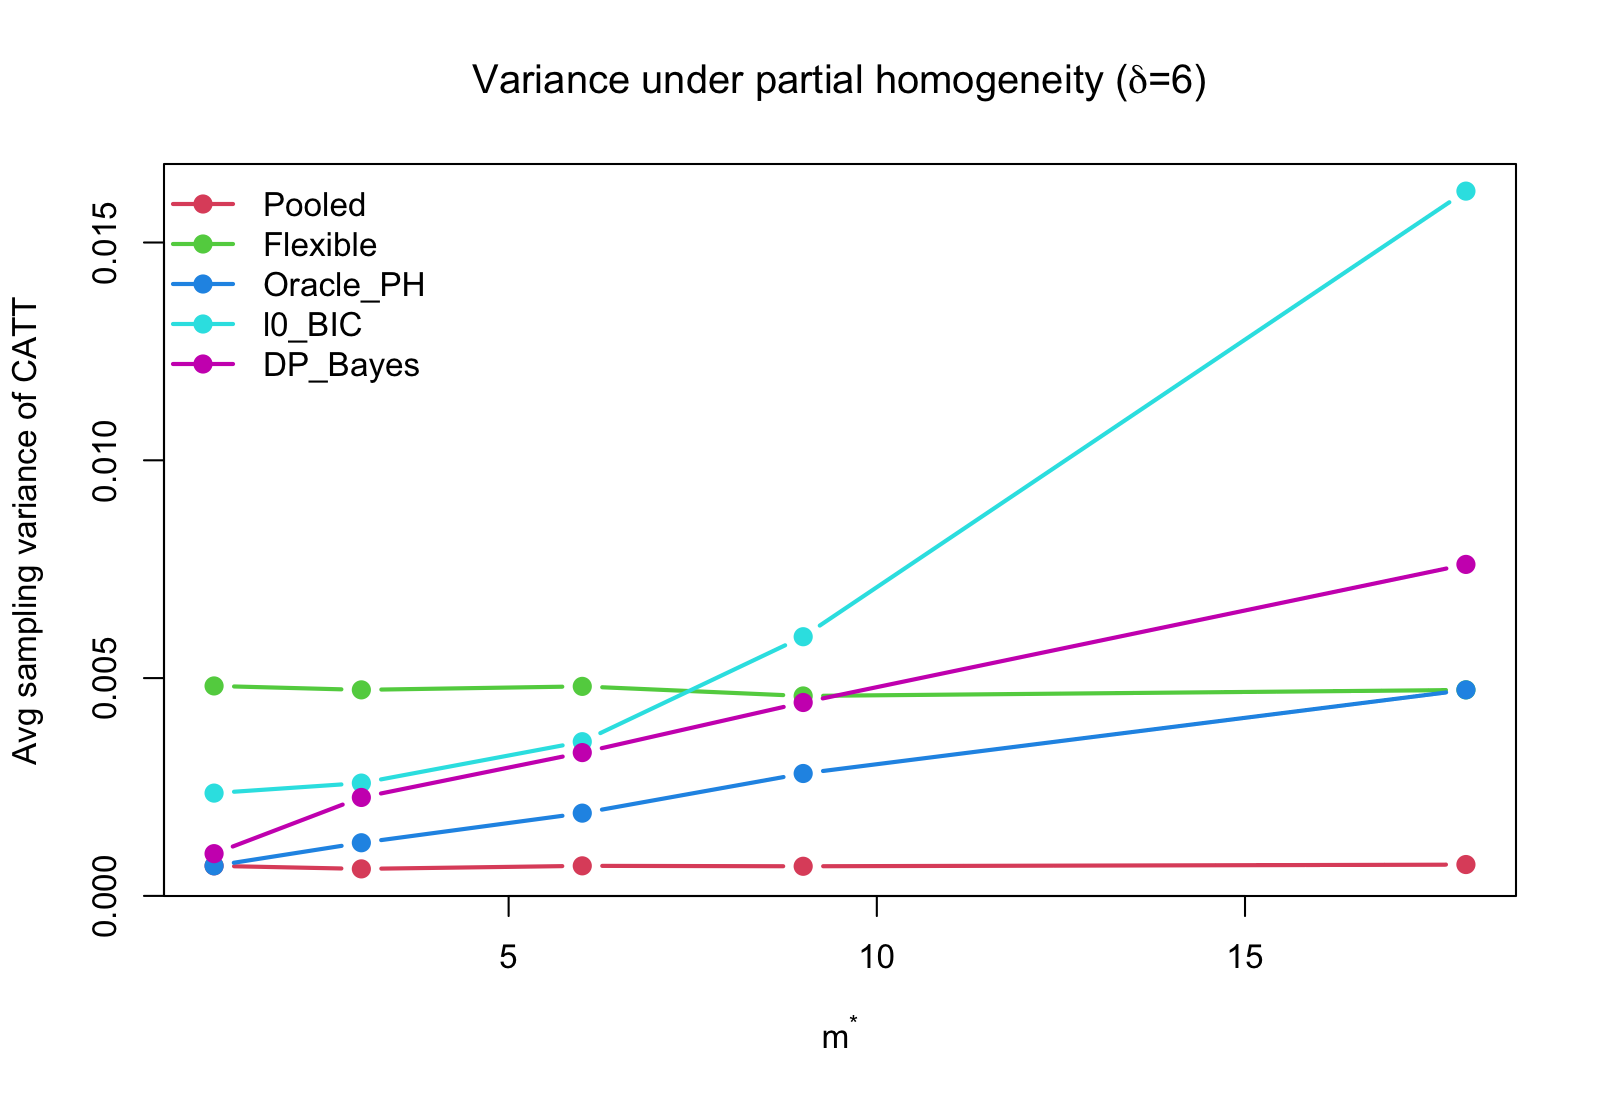
\includegraphics[width=0.7\linewidth]{variance_vs_mstar.png}
  \caption{Average sampling variance of the cohort-time estimates against the true
  number of distinct effects $m^{\ast}$ ($\delta=6$). The $\ell_0$ and DP
  estimators track the infeasible oracle in the partial-homogeneity region and
  revert to flexible TWFE as $m^{\ast}\to K$.}
  \label{fig:sim:var}
\end{figure}

The realized gain depends on how well separated the distinct effects are, exactly
as the recovery interval of Proposition~\ref{prop:threshold} suggests.
Table~\ref{tab:sim:sep} fixes $m^{\ast}=6$ and varies $\delta$.

\begin{table}[H]
  \centering
  \caption{Effect of separation $\delta$ on precision and recovery,
  $m^{\ast}=6$. Variance ratio to flexible and ARI. $500$ replications.}
  \label{tab:sim:sep}
  \small
  \begin{tabular}{lcccccc}
    \toprule
    & \multicolumn{2}{c}{$\delta=3$} & \multicolumn{2}{c}{$\delta=6$}
    & \multicolumn{2}{c}{$\delta=12$} \\
    \cmidrule(lr){2-3}\cmidrule(lr){4-5}\cmidrule(lr){6-7}
    Method & Var ratio & ARI & Var ratio & ARI & Var ratio & ARI \\
    \midrule
    Oracle PH & 0.40 & 1.00 & 0.40 & 1.00 & 0.40 & 1.00 \\
    $\ell_0$-PH  & 1.47 & 0.54 & 0.74 & 0.95 & 0.41 & 1.00 \\
    Bayes-PH  & 1.19 & 0.46 & 0.69 & 0.88 & 0.46 & 0.93 \\
    \bottomrule
  \end{tabular}
\end{table}

When the effects are close ($\delta=3$) the partition cannot be recovered
reliably (ARI $\approx 0.5$) and the selection noise erases, indeed reverses, the
variance advantage, and both feasible estimators are then less precise than
flexible TWFE. As separation grows the gap to the oracle closes, and at
$\delta=12$ the feasible $\ell_0$-PH estimator essentially attains the oracle
variance reduction (0.41 versus 0.40) with near-perfect recovery.
Figure~\ref{fig:sim:sep} shows the monotone relationship. The practical message
is that the methods deliver their promised gains when heterogeneity is
``clumpy'', a modest number of well-separated effect levels, and should not
be expected to when the effects form a near-continuum. A secondary but useful
observation is that the Bayes-PH estimator is the more robust of the two, since in the
hard regimes ($\delta=3$, or $\delta=6$ with the fine $m^{\ast}=9$ partition) its
variance ratio stays at or below one, whereas the $\ell_0$-PH estimator, which
commits to a single partition, has a heavier tail and can exceed one.

\begin{figure}[H]
  \centering
  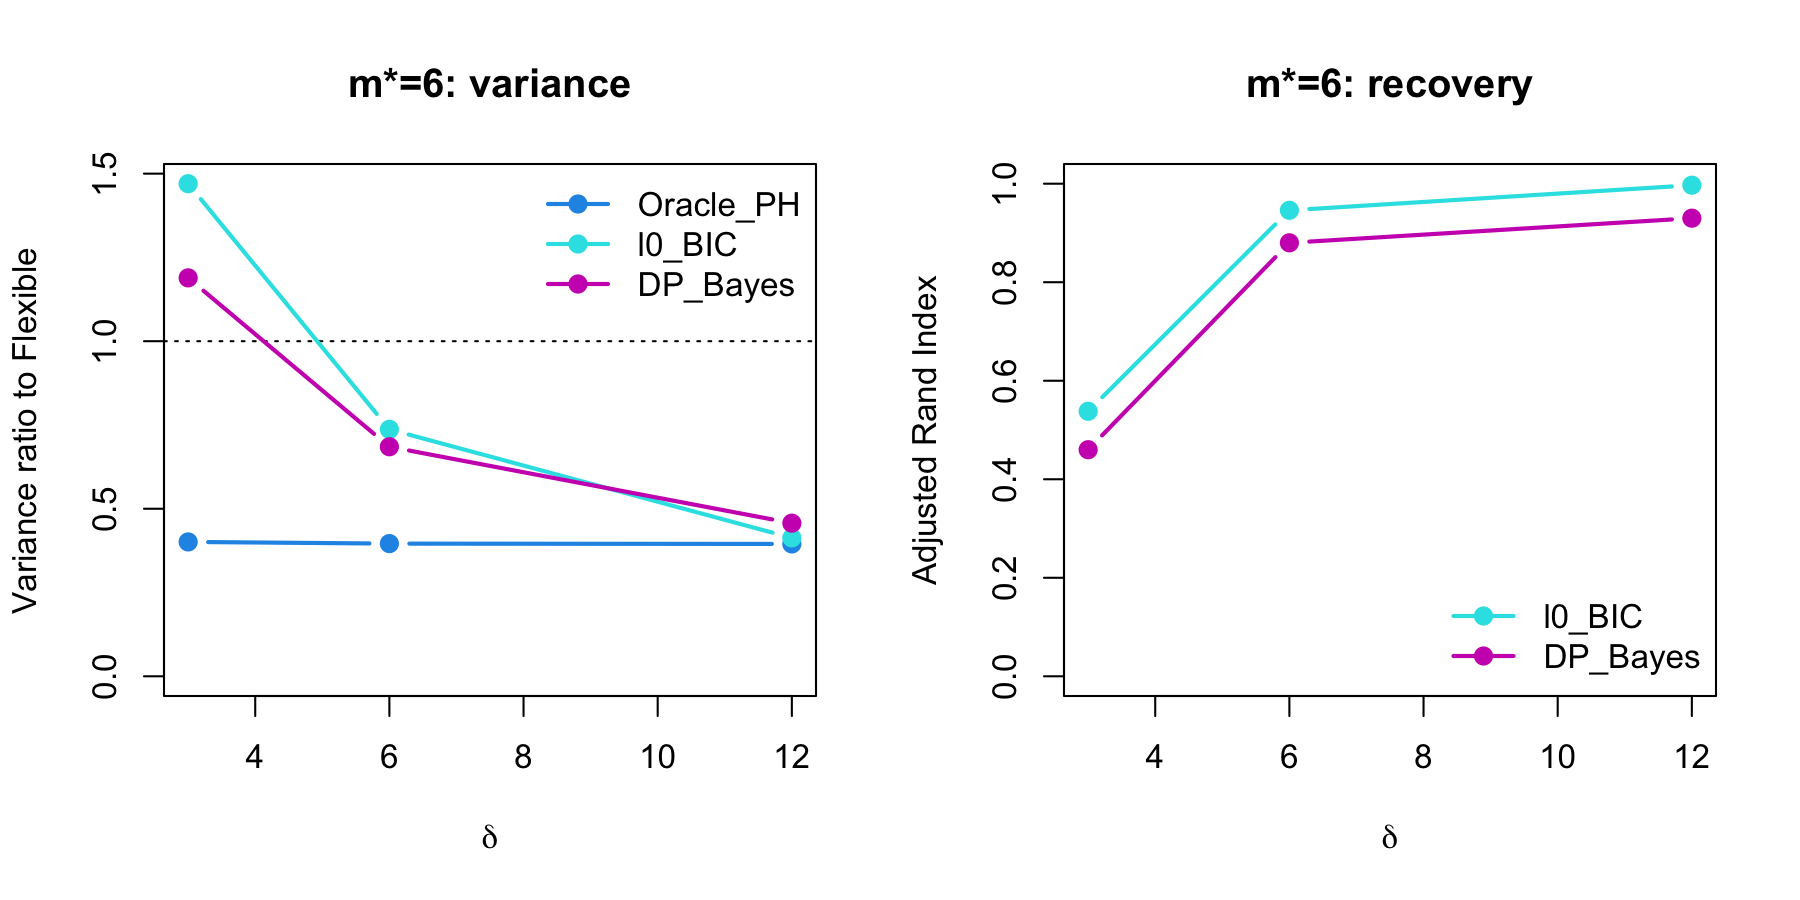
\includegraphics[width=\linewidth]{separation_vs_delta.png}
  \caption{Precision (left) and partition recovery (right) as functions of the
  separation $\delta$, at $m^{\ast}=6$. The variance advantage over flexible TWFE
  (values below the dashed line) is realized only once the effects are separated
  enough to be recovered.}
  \label{fig:sim:sep}
\end{figure}

\subsection{Honest inference: coverage}
\label{sec:sim:cov}

Table~\ref{tab:sim:cov} evaluates the calibration of $95\%$ intervals at
$m^{\ast}=6$, $\delta=6$, reporting coverage and average length for the
cohort-time effects and for the overall ATT. For the $\ell_0$-PH estimator we
report the plug-in interval that treats the selected partition as fixed. The
Bayes-PH interval is the $2.5$--$97.5\%$ posterior credible interval.

\begin{table}[H]
  \centering
  \caption{Coverage and average length of nominal $95\%$ intervals at
  $m^{\ast}=6$, $\delta=6$; targets are the true CATTs and the true ATT. Oracle PH
  is infeasible. $500$ replications.}
  \label{tab:sim:cov}
  \small
  \begin{tabular}{lcccc}
    \toprule
    & \multicolumn{2}{c}{CATT} & \multicolumn{2}{c}{ATT} \\
    \cmidrule(lr){2-3}\cmidrule(lr){4-5}
    Method & Coverage & Length & Coverage & Length \\
    \midrule
    Pooled                 & 0.05 & 0.10 & 0.05 & 0.10 \\
    Flexible               & 0.96 & 0.27 & 0.95 & 0.12 \\
    Oracle PH              & 0.95 & 0.17 & 0.95 & 0.11 \\
    $\ell_0$-PH             & 0.91 & 0.17 & 0.94 & 0.11 \\
    Bayes-PH               & 0.94 & 0.20 & 0.95 & 0.11 \\
    \bottomrule
  \end{tabular}
\end{table}

The pooled intervals collapse (coverage $0.04$--$0.05$): they are short but
centered on a biased estimand. The flexible and oracle intervals are correctly
calibrated, the oracle being much shorter, and they bracket the feasible
estimators. The Bayes-PH credible intervals attain near-nominal coverage
($0.94$ for the CATTs, $0.95$ for the ATT) at a length between oracle and
flexible, honest and informative uncertainty. The $\ell_0$-PH interval is
only mildly anti-conservative here ($0.91$ CATT, $0.94$ ATT): at this separation
the correct partition is recovered often enough that the conditional-on-selection
distortion is small.\footnote{A natural alternative removes this distortion by
sample splitting, selecting the partition on one half of the units and computing
coefficients and standard errors on the other. It does not help, its coverage is
in fact lower ($0.74$ CATT, $0.90$ ATT). Splitting halves the sample, which
degrades recovery, and a wrongly merged partition then injects a specification
bias that a correctly sized standard error cannot undo.} Honest uncertainty under
partition selection thus comes not from adjusting the variance but from averaging
over the partition, which is what the DP posterior does.
It is also worth noting what does drive the result. The calibration hinges on
using the exact cross-cell covariance of the cohort-time estimates
(Remark~\ref{rem:sigma}), whereas the treatment of $\sigma^2$ is immaterial. The
full Bayesian sampler draws $\sigma^2$ from its inverse-gamma full conditional, and
holding it fixed at a plug-in value gives essentially the same coverage and
interval length (Appendix~\ref{app:sigma}).

\subsection{Solution paths}
\label{sec:sim:path}

Figure~\ref{fig:sim:path} traces the bias-variance trade-off as a function of
the regularization strength, for $\ell_0$-PH along the agglomeration path indexed by the
number of groups $m$ (small $m$ = strong penalty), and for DP across the
concentration $\alpha$. Two features are worth emphasizing. First, the overall
ATT is remarkably robust to over-pooling, where its bias stays small
($\lesssim 0.015$) across the entire $\ell_0$ path down to $m=3$ and only spikes
once the path collapses toward a single group ($|$bias$|=0.10$ at $m=1$), while
the CATT variance falls as cells are pooled. The aggregate thus tolerates a wide
range of penalties, whereas the cohort-time effects require getting the partition
approximately right, the CATT variance is minimized near the true $m=6$ and
inflates when the path is forced into wrong merges. Second, the DP path is nearly
flat in $\alpha$: both the ATT bias and variance barely move over
$\alpha\in\{1,\dots,30\}$, so the practitioner's choice of concentration has
little effect on the reported estimates. The mean BIC-selected number of groups
($\approx 6.2$) sits in the flat, low-bias region of the $\ell_0$ path, confirming
that the plateau in $\hat m$ is a serviceable tuning diagnostic.

\begin{figure}[H]
  \centering
  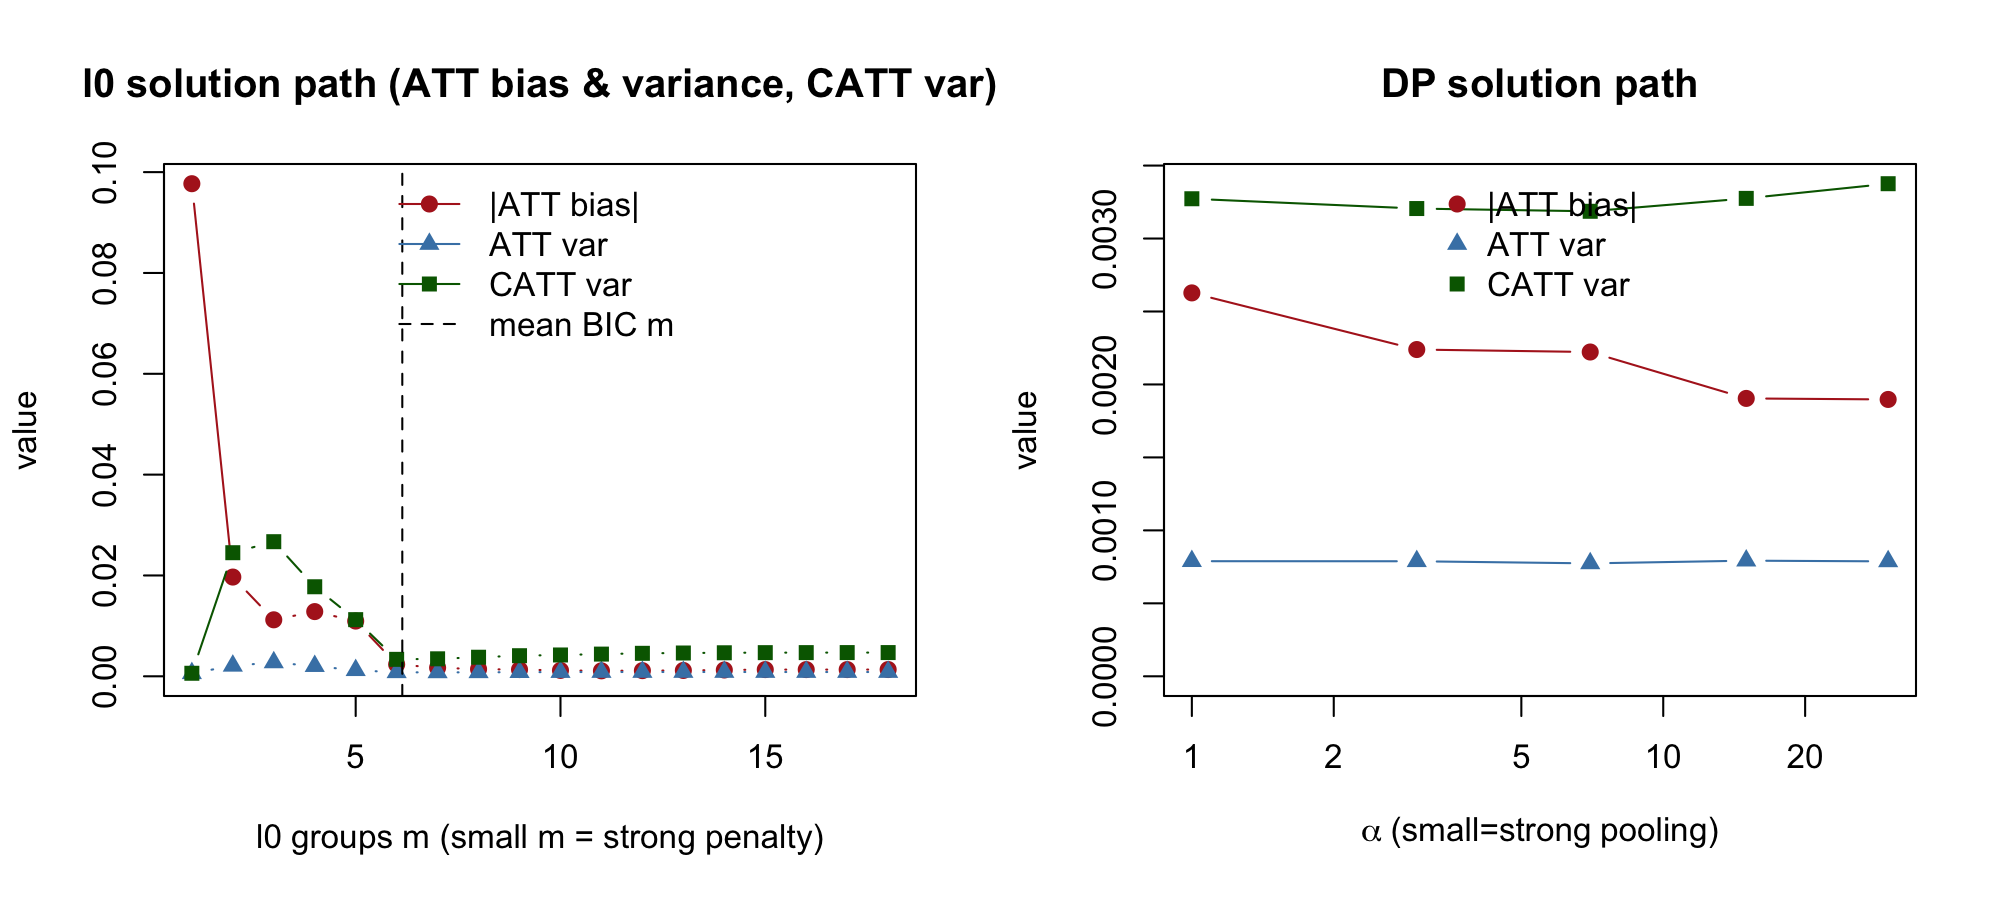
\includegraphics[width=\linewidth]{solution_paths.png}
  \caption{Solution paths at $m^{\ast}=6$, $\delta=6$. Left: $\ell_0$, indexed by
  the number of groups $m$ (dashed line = mean BIC selection). Right: DP, indexed
  by the concentration $\alpha$ (log scale). The overall ATT bias (red) stays
  near zero across a wide range while the CATT variance (green) falls with
  pooling.}
  \label{fig:sim:path}
\end{figure}

% =============================================================================
% 6. EMPIRICAL APPLICATION  (kept as in the working draft; to be finalized)
% =============================================================================
\section{Empirical Applications}
\label{sec:empirical_application}

We present two applications that exhibit the two regimes the method is built for, one where the cohort-time effects carry recoverable heterogeneity and one where they are indistinguishable from a common value.

\subsection{Minimum Wages and Teen Employment: Recovering Partial Homogeneity}
\label{sec:cs_application}

We revisit the county-level analysis of minimum wages and teen employment from
\citet{callaway2021}, using their publicly available panel of $500$ U.S.\
counties observed over $2003$--$2007$, with cohorts first raising the minimum
wage in $2004$, $2006$, and $2007$ and a not-yet-treated control group. We
estimate the $K=7$ post-treatment cohort-time effects $\mathrm{ATT}(g,t)$ with the
\citet{callaway2021} estimator and take their exact joint covariance
$\hat\Sigma$ from the estimator's influence functions. Because the cells share
counties, $\hat\Sigma$ is non-diagonal; as in the simulations, we use it exactly
in both estimators, and the DP posterior draws use the corresponding
Gauss--Markov posterior (Remark~\ref{rem:sigma}).

Unlike a homogeneous design, here there is real structure to recover, as the
cross-cell dispersion of the estimates ($0.050$) is more than twice the typical
standard error ($0.022$), a signal-to-noise ratio of $2.25$ that places the
application in the recoverable region of Section~\ref{sec:sim}.
Table~\ref{tab:cs} reports the seven effects, the $\ell_0$ grouping selected by
BIC, and the per-cell variance reduction.

\begin{table}[H]
    \centering
    \caption{Cohort-time effects on log teen employment, \citet{callaway2021}
    data. $\mathrm{ATT}(g,t)$ and its standard error; the BIC-selected $\ell_0$
    group and grouped effect; and the ratio of the $\ell_0$-grouped variance to
    the flexible variance for each cell (lower = more precise).}
    \label{tab:cs}
    \small
    \begin{tabular}{lccccc}
        \toprule
        cohort:year & $\mathrm{ATT}(g,t)$ & SE & $\ell_0$ group & grouped effect & var.\ ratio \\
        \midrule
        2004:2004 & $-0.019$ & 0.022 & 1 & $-0.029$ & 0.28 \\
        2006:2007 & $-0.041$ & 0.020 & 1 & $-0.029$ & 0.33 \\
        2007:2007 & $-0.026$ & 0.017 & 1 & $-0.029$ & 0.49 \\
        2004:2005 & $-0.078$ & 0.030 & 2 & $-0.087$ & 0.77 \\
        2004:2007 & $-0.101$ & 0.034 & 2 & $-0.087$ & 0.61 \\
        2004:2006 & $-0.136$ & 0.035 & 3 & $-0.140$ & 0.78 \\
        2006:2006 & $+0.005$ & 0.016 & 4 & $+0.011$ & 0.78 \\
        \bottomrule
    \end{tabular}
\end{table}

The $\ell_0$-PH estimator collapses the seven cells into four effect levels: a
near-zero group containing the $2004$ impact effect and the recent cohorts'
effects, the $2004$ cohort's larger mature effects, its peak, and the lone
positive cell. Pooling roughly halves the variance of the cells that share a
group (the near-zero group's variance ratios are $0.28$--$0.49$), and even the
singleton cells gain precision because the Gauss--Markov estimator borrows across
the correlated cells. The overall (cohort-size-weighted) average effect is
essentially unchanged and slightly more precise, $-0.040$ (SE $0.012$) under
the flexible estimator versus $-0.039$ (SE $0.012$) under $\ell_0$, so the
substantive conclusion of a roughly $4\%$ teen-employment reduction is preserved
while the estimates are summarized by a handful of interpretable effect levels.
These point estimates agree on the headline, but both condition on a single
grouping, and the Dirichlet-Process posterior that follows both gauges how firmly
that grouping is identified and, given the small number of cells, shows how much
the overall summary can move once that conditioning is relaxed.

The DP posterior sharpens the interpretation by quantifying which groupings
are certain. Figure~\ref{fig:cs} plots the effects colored by $\ell_0$ group and
the posterior co-clustering matrix. The near-zero cells co-cluster with high
probability ($0.77$--$0.90$), so the ``small effect'' group is a robust feature;
the $2004$ cohort's dynamic cells co-cluster only moderately ($0.56$--$0.70$),
correctly signaling that the finer split of its smooth ramp is uncertain rather
than a firm partition. This is the honest reading the co-clustering is meant to
deliver, a reliable coarse structure with calibrated uncertainty about the finer
detail.

\begin{figure}[H]
    \centering
    \begin{subfigure}{0.54\linewidth}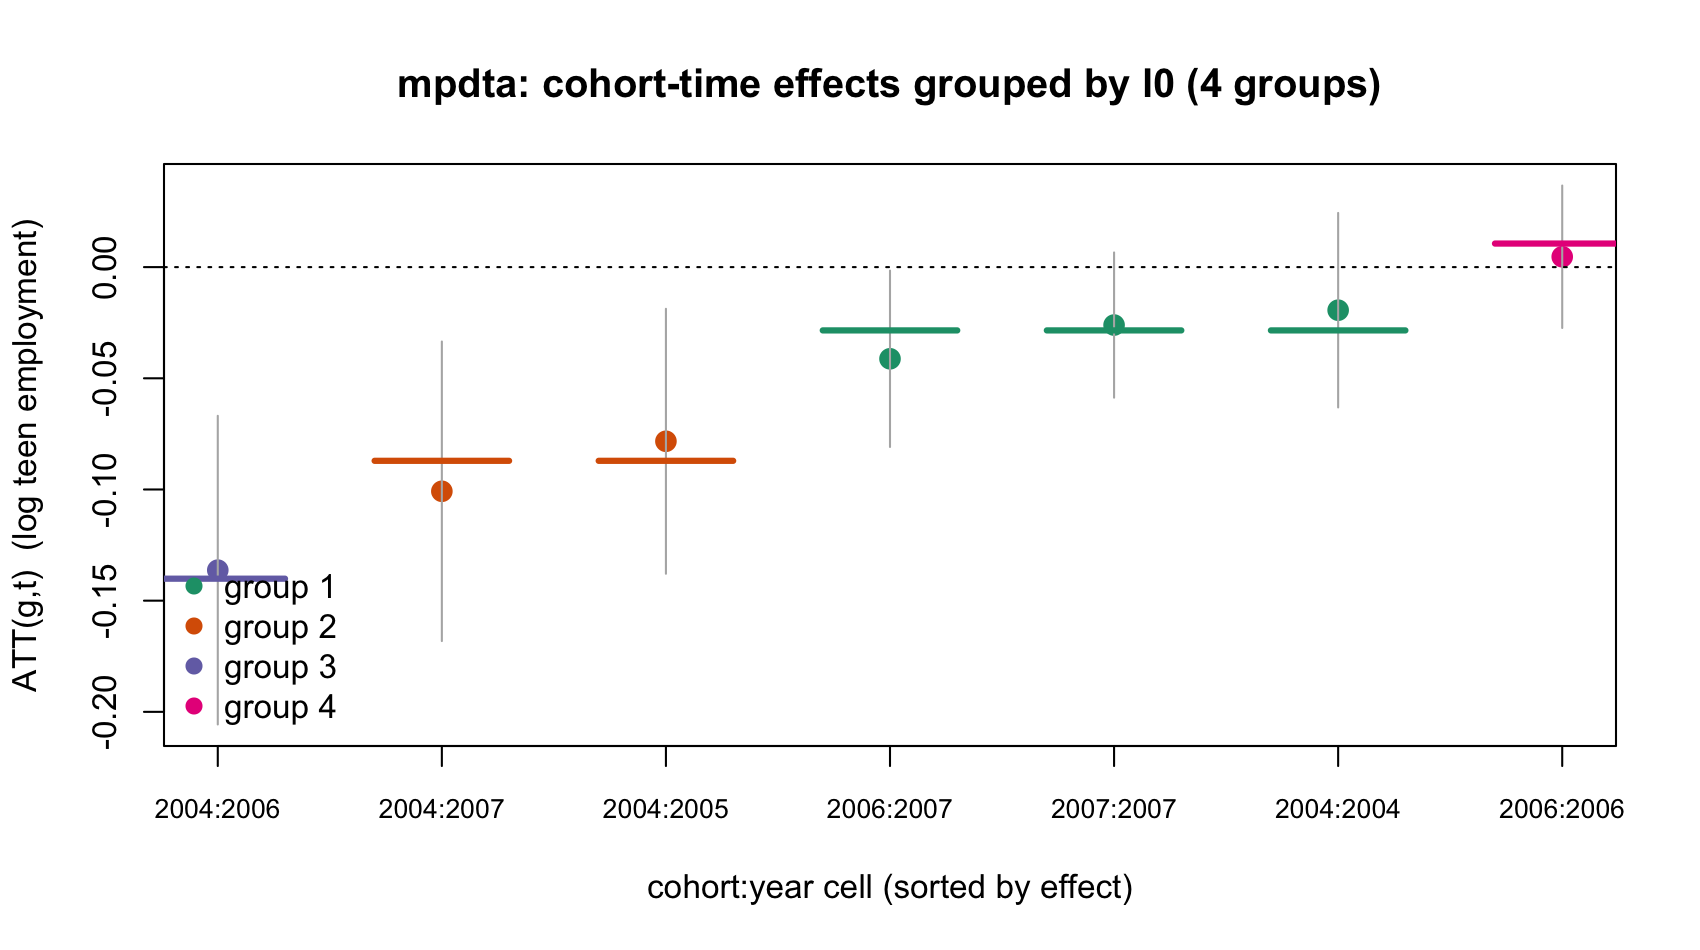
\includegraphics[width=\linewidth]{mpdta_effects.png}\end{subfigure}
    \hfill
    \begin{subfigure}{0.44\linewidth}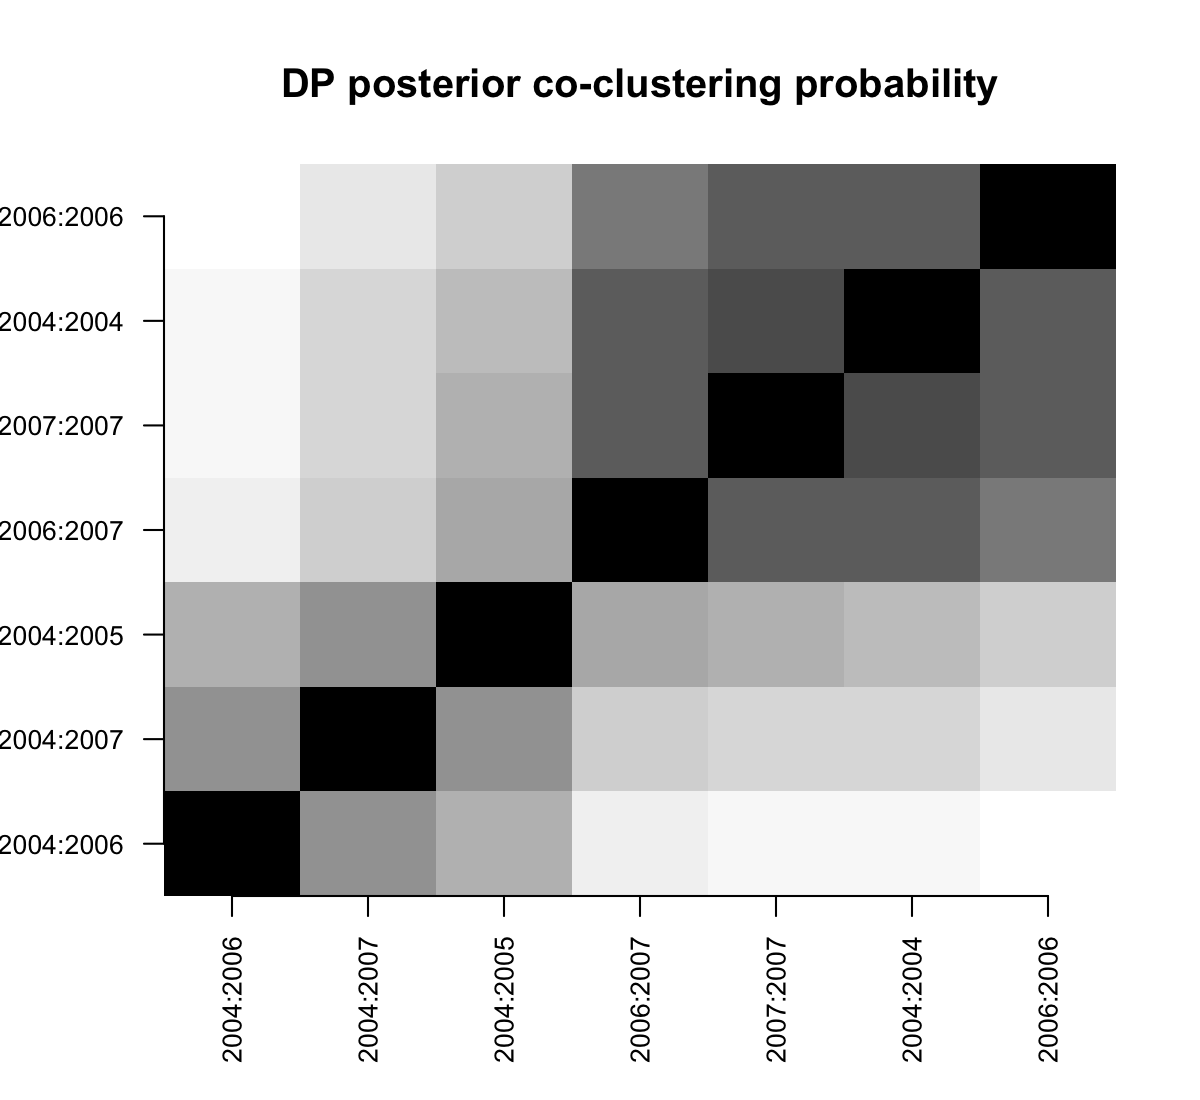
\includegraphics[width=\linewidth]{mpdta_coclust.png}\end{subfigure}
    \caption{Left: the seven cohort-time effects (with $95\%$ intervals) colored
    by $\ell_0$ group, horizontal bars mark the grouped effects. Right: the DP
    posterior co-clustering probabilities; darker cells co-cluster more often.}
    \label{fig:cs}
\end{figure}

Because the number of cells is small, the DP overall effect, unlike the flexible and $\ell_0$-PH point estimates, is sensitive to the concentration $\alpha$. Figure~\ref{fig:cs_alpha} traces the population-weighted effect and its $95\%$ credible band across $\alpha$ from $0.1$ to $100$, against the fully pooled ($-0.010$) and flexible ($-0.040$) anchors. The effect slides monotonically from about $-0.014$ under heavy pooling to about $-0.037$ as $\alpha$ grows and the model approaches the flexible fit, and it is bounded away from zero only for $\alpha \gtrsim 2$. Rather than fix $\alpha$, we report the whole path. As a reference point, a BIC pass on the agglomeration path selects four groups, which the prior's expected group count matches at $\alpha \approx 13$ (panel b), where the DP effect is about $-0.03$ and close to the flexible estimate. We offer this only as a suggestion. Choosing $\alpha$ from the data turns the prior into a data-dependent object, with the usual consequences of empirical Bayes (understated posterior uncertainty and a double use of the data), so we prefer to show the sensitivity rather than commit to a single value.

\begin{figure}[H]
    \centering
    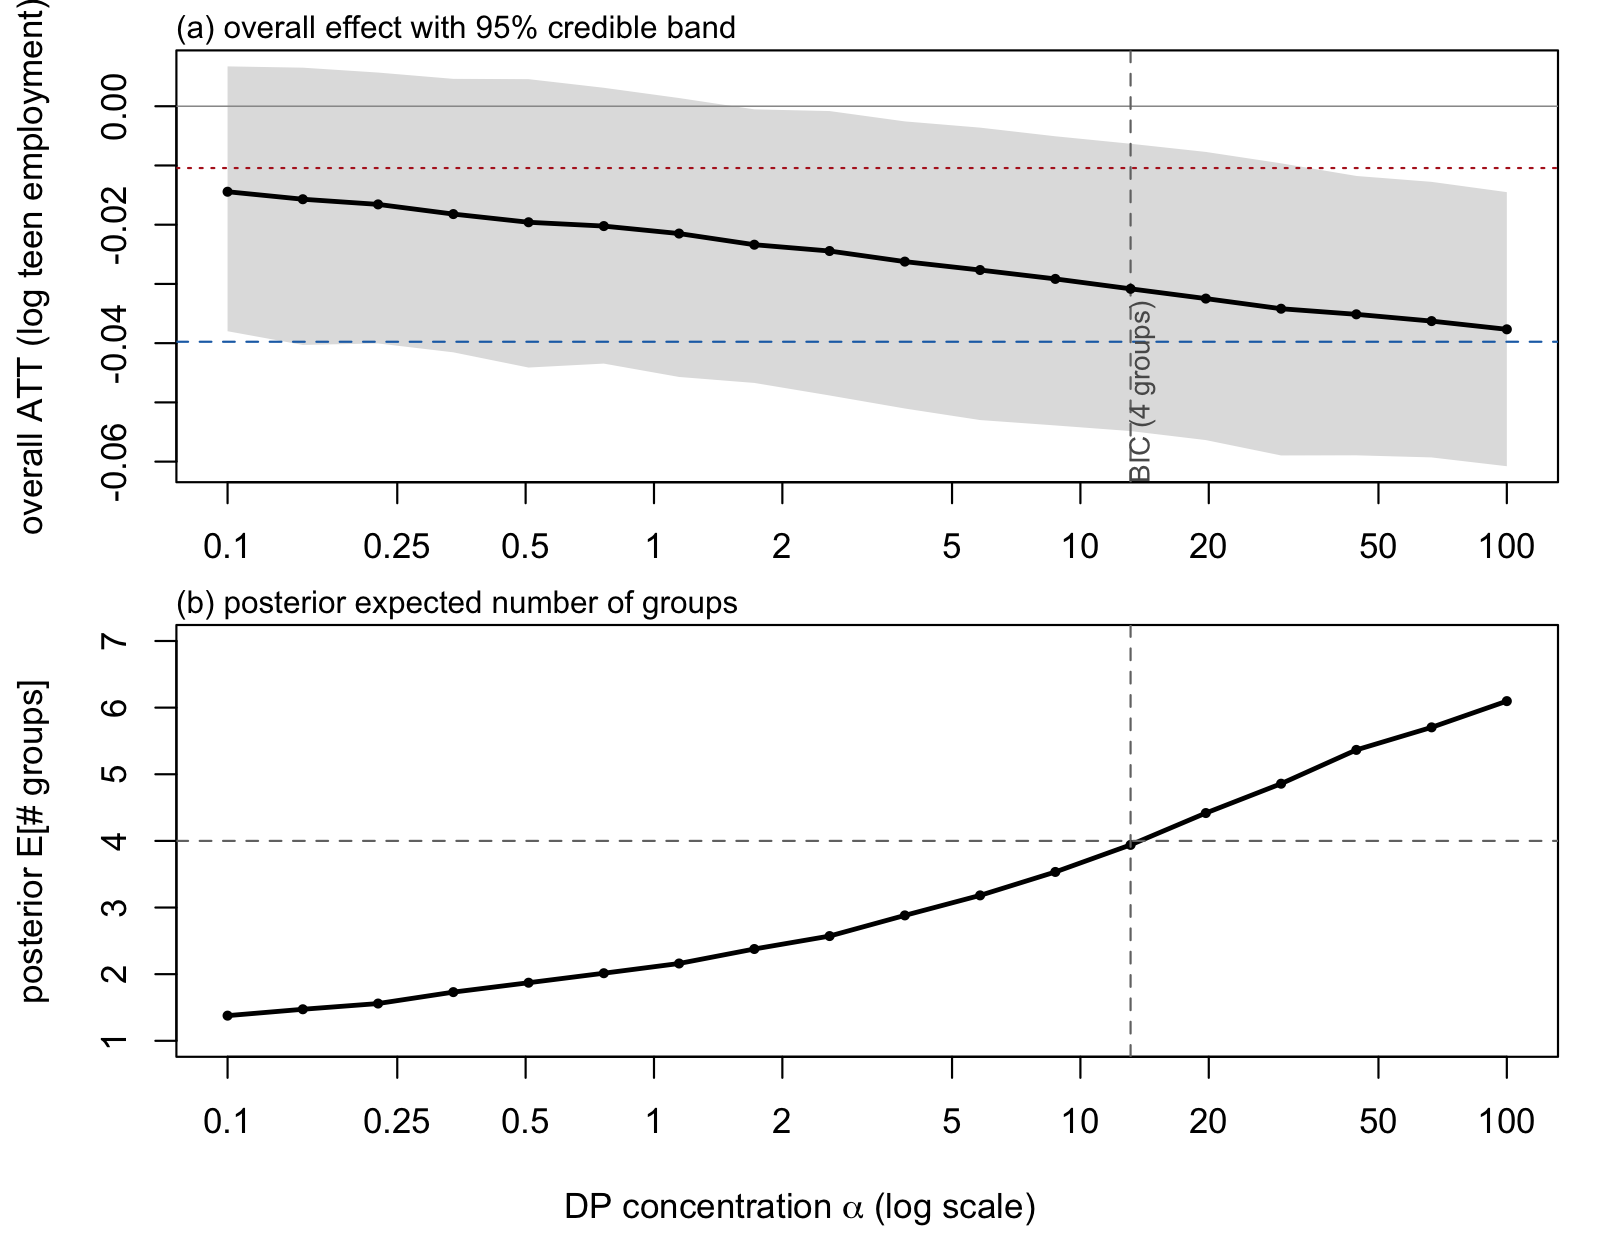
\includegraphics[width=0.8\linewidth]{mpdta_alpha.png}
    \caption{Sensitivity of the \citet{callaway2021} overall effect to the DP
    concentration $\alpha$. Panel (a), the population-weighted overall ATT (solid)
    with its $95\%$ credible band (shaded), against the fully pooled (red dotted,
    $-0.010$) and flexible (blue dashed, $-0.040$) benchmarks. Panel (b), the
    posterior expected number of groups. The vertical line marks $\alpha \approx 13$,
    where the prior's expected group count equals the four groups selected by BIC
    on the agglomeration path.}
    \label{fig:cs_alpha}
\end{figure}

The dynamic (event-study) aggregation in Figure~\ref{fig:cs_dyn} clarifies what
the estimators are grouping. The effect on teen employment is small at impact
(event time $0$, $-0.019$) and grows over the horizon to $-0.054$, $-0.136$, and
$-0.101$ at event times $1$ through $3$, the familiar pattern of a
minimum-wage effect that accumulates over several years. Because only the $2004$
cohort is observed at the longer horizons, its later cells carry the large
effects while the impact-year effects are small and similar across cohorts. The
partial homogeneity the method recovers is, in this application, largely the
homogeneity of the short-run response across cohorts, with the accumulating
longer-run effects kept separate. The pre-treatment coefficients are small
(event times $-2$ and $-1$), with a modest positive value at the longest lead
that is identified off a single early cohort.

\begin{figure}[H]
    \centering
    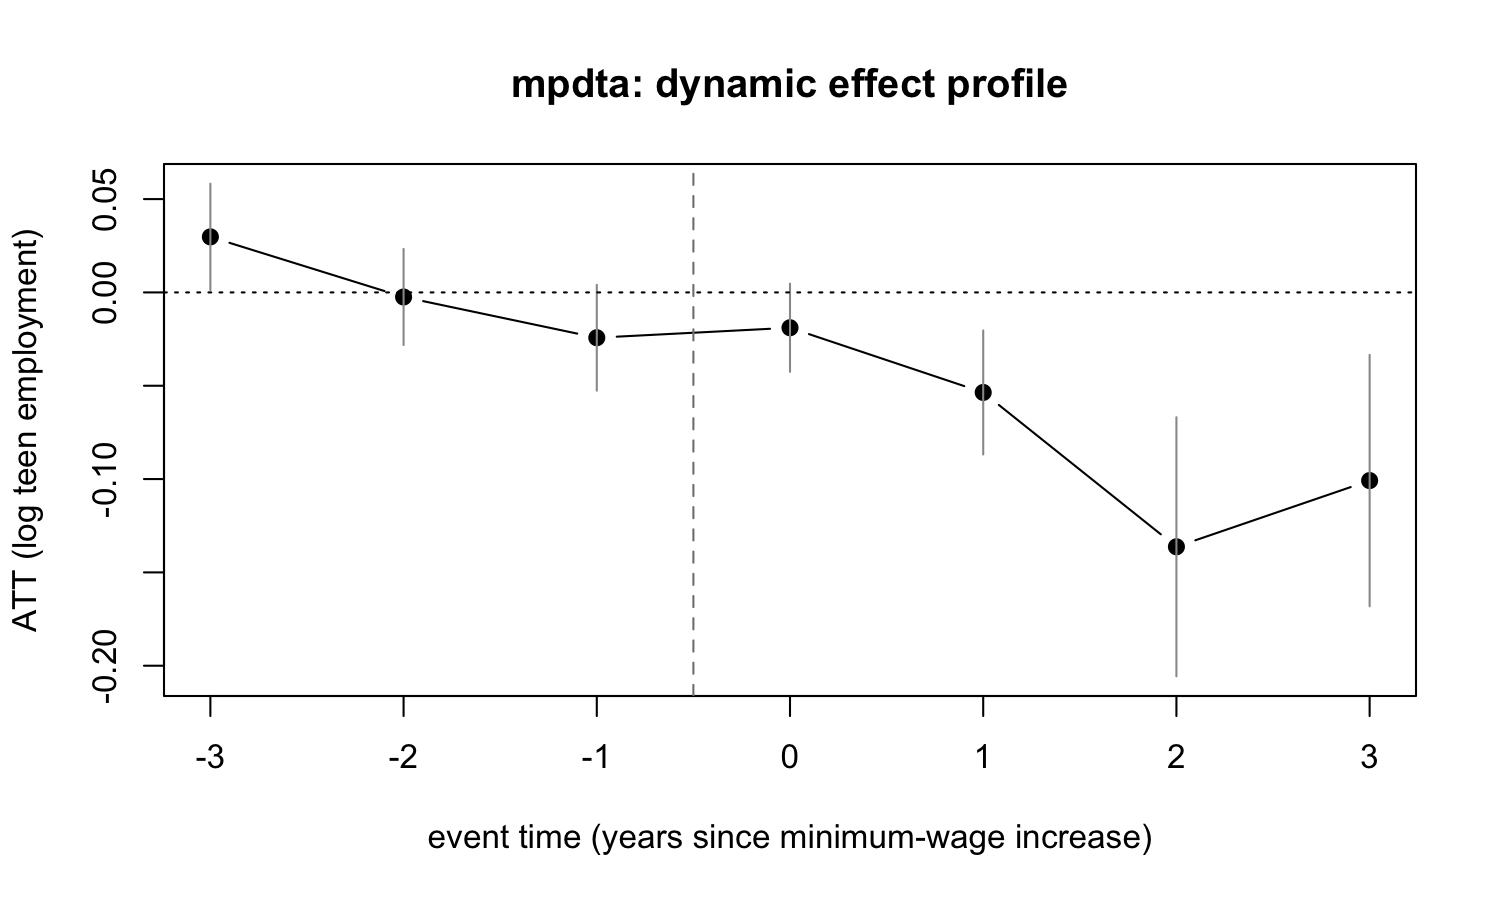
\includegraphics[width=0.62\linewidth]{mpdta_dynamic.png}
    \caption{Dynamic (event-study) aggregation of the \citet{callaway2021}
    effects: the teen-employment effect is near zero at impact and builds over
    event time. Pre-treatment coefficients (left of the dashed line) are small.}
    \label{fig:cs_dyn}
\end{figure}

\subsection{Minimum Wages and Low-Wage Jobs: A Specification Test}
\label{sec:cengiz_application}

Our second application is the influential study of minimum wages and low-wage
jobs by \citet{cengiz2019}, which estimates the employment effect of $138$
state-level minimum wage increases between $1979$ and $2016$ using a ``stacked''
event-study design. Here the method plays the complementary role of a
specification test.

\subsubsection{Context and Stacked Event-Study Design}

In the stacked design, a separate dataset (a ``stack'' or ``event'') is created for each of the $E = 138$ minimum wage hikes. Each stack $g \in \{1, \dots, E\}$ contains the treated state and a set of clean control states observed over a 5-year window around the policy implementation. The stacks are then appended together.

The authors' baseline specification is a fully pooled TWFE regression on the stacked data, which imposes a single, homogeneous treatment effect across all 138 events:
\begin{equation} \label{eq:pooled_cengiz}
    Y_{itg} = \alpha_{ig} + \gamma_{tg} + \theta \cdot D_{itg} + \epsilon_{itg},
\end{equation}
where $Y_{itg}$ is the employment outcome for state $i$ at time $t$ in stack $g$. The terms $\alpha_{ig}$ and $\gamma_{tg}$ are state-by-stack and time-by-stack fixed effects, ensuring that treated units are only compared to control units within their specific sub-experiment. $D_{itg}$ is an indicator equal to 1 if state $i$ is treated in stack $g$ in the post-treatment period. Under this specification, the authors report a near-zero average effect on net low-wage employment.

However, as established in Section~\ref{sec:problem}, this pooled estimator $\hat{\theta}$ is efficient but biased if the true treatment effects are heterogeneous. To allow for heterogeneity, we relax Equation~\ref{eq:pooled_cengiz} into a fully flexible Interacted TWFE (ITWFE) model, assigning a distinct Cohort-Average Treatment Effect on the Treated (CATT), $\tau_g$, to each event:
\begin{equation} \label{eq:flexible_cengiz}
    Y_{itg} = \alpha_{ig} + \gamma_{tg} + \sum_{g=1}^{E} \tau_g \left( D_{itg} \times \mathbb{I}\{event = g\} \right) + \epsilon_{itg}
\end{equation}

Because the design matrix of Equation~\ref{eq:flexible_cengiz} is block-diagonal, the estimation of each $\hat{\tau}_g$ is perfectly separable. While this flexible model is unbiased, relying strictly on state-level variation yields highly noisy estimates for individual events.

To recover the latent structure, we apply our $\ell_0$-penalized estimator. We select the optimal partition of the 138 minimum wage effects by minimizing the penalized residual sum of squares:
\begin{equation} \label{eq:penalized_cengiz}
    \min_{\boldsymbol{\tau}, \boldsymbol{\alpha}, \boldsymbol{\gamma}} \left\{ \sum_{g=1}^{E} \sum_{i,t} \left( Y_{itg} - \alpha_{ig} - \gamma_{tg} - D_{itg} \tau_g \right)^2 + \lambda \sum_{j < k} \mathbb{I}(\tau_j \neq \tau_k) \right\},
\end{equation}
where $\lambda$ is the hyperparameter determining the threshold for model parsimony. The penalty forces states with sufficiently similar independent estimates to share a single coefficient, achieving partial homogeneity without imposing the strict global restriction of Equation~\ref{eq:pooled_cengiz}.

\subsubsection{Baseline Replication and Data Hygiene}

Before applying the penalized estimator to explore latent heterogeneity, we first replicate the fully pooled TWFE specification from \citet{cengiz2019} to establish a baseline. Table~\ref{tab:baseline_replication} demonstrates that our replication sample accurately recovers the primary pooled estimates reported by the authors. The pooled model implies a near-zero average net effect on low-wage employment, driven by the destruction of jobs below the new minimum wage ($\Delta b$) being largely offset by the ``bunching'' of new compliance jobs at or slightly above the new minimum wage ($\Delta a$).

\begin{table}[H]
    \centering
    \caption{Baseline Pooled ITWFE Replication}
    \label{tab:baseline_replication}
    \begin{tabular}{lc}
        \toprule
        \textbf{Employment Outcome} & \textbf{Pooled Estimate} \\
        \midrule
        Missing Jobs ($\Delta b$) & $-0.016^{***}$ \\
        Excess Jobs ($\Delta a$) & $0.019^{***}$ \\
        Net Employment Change & $0.003$ \\
        \bottomrule
    \end{tabular}
    \vspace{0.1cm}
    \begin{minipage}{0.7\textwidth}
        \small Note: Estimates represent the change in employment as a fraction of the affected workforce. These pooled point estimates closely mirror the benchmark findings of the original study, suggesting a negligible average disemployment effect.
    \end{minipage}
\end{table}

While the pooled model provides a stable average, estimating Equation~\ref{eq:flexible_cengiz} flexibly for all 138 independent events reveals severe localized sampling anomalies. Because the employment effects are normalized by $\bar{b}_{-1}$ (the share of the state's workforce earning below the new minimum wage in the year prior to the hike), regions with very thin survey samples can produce a denominator approaching zero. Dividing the raw job counts by a near-zero denominator causes the resulting percentage estimate to artificially explode to economically impossible magnitudes.

A handful of events yield mathematically anomalous net percentage effects (exceeding several hundred percent of the affected workforce) for exactly this reason. To sidestep the near-zero-denominator problem, our specification analysis below summarizes each event by its average post-treatment event-study coefficient on affected employment rather than by the ratio-normalized percentage effect; the event-study coefficient is well behaved (its cross-event standard deviation is $0.005$, with no explosive outliers).

\subsubsection{Specification Analysis: Is the Null Effect Homogeneous?}
\label{sec:cengiz:spec}

We obtain the $E = 138$ event-level effects from the authors' Harvard Dataverse replication package for \citet{cengiz2019}, summarizing event $g$ by $\hat\tau_g$, the average of its post-treatment event-study coefficients on affected employment (event times $0$ through $4$). Before selecting a specification, we ask whether there is any heterogeneity to recover. The design provides an internal noise gauge, since under no-anticipation the pre-treatment coefficients have expectation zero, so their cross-event dispersion measures the per-event sampling noise. We find a pre-treatment (noise) standard deviation of $0.0065$, which exceeds the post-treatment cross-event spread of $0.0050$. The implied signal-to-noise ratio is $0.77$, and the variance decomposition attributes essentially $0\%$ of the cross-event variation in employment effects to genuine heterogeneity, so the 138 event effects are statistically indistinguishable from a common value.

This places the application squarely in the low-separation regime that Section~\ref{sec:sim} identifies as the boundary of reliable recovery, and the estimators behave accordingly. The BIC-tuned $\ell_0$-PH estimator splits the events into five effect-ordered bands (of sizes $51$, $47$, $36$, $3$, $1$), and the Bayes-PH estimator returns between $2.7$ groups (parsimonious prior, $\alpha=1$) and $7.6$ groups ($\alpha=5$). As our simulations show, at a signal-to-noise ratio below one these ``groups'' are quantiles of noise rather than genuine effect clusters, and should not be interpreted as evidence of systematic heterogeneity; indeed, the formal test above finds none. The disagreement between the two estimators is itself a symptom of the regime.

What is robust, and what matters for the applied conclusion, is that the overall average effect is invariant to the specification. Table~\ref{tab:cengiz:att} reports it, showing that the pooled, $\ell_0$, and Bayes-PH estimates of the population-weighted average employment effect are all near zero and mutually indistinguishable, and the DP posterior credible interval excludes economically meaningful disemployment. Allowing for arbitrary event-level heterogeneity does not overturn the near-zero net-employment finding of \citet{cengiz2019}; it confirms that the pooled specification is adequate for the aggregate. Figure~\ref{fig:cengiz} displays the 138 flexible event effects with the pooled effect superimposed.

\begin{table}[H]
    \centering
    \caption{Overall employment effect under alternative specifications, Cengiz et al.\ (2019) events. Effects are average post-treatment coefficients on affected employment (population-weighted for the aggregate). The Bayes-PH interval is the $95\%$ posterior credible interval.}
    \label{tab:cengiz:att}
    \small
    \begin{tabular}{lcc}
        \toprule
        Specification & Groups & Overall effect \\
        \midrule
        Pooled (single effect)      & $1$    & $0.0015$ \\
        Flexible (per event)        & $138$  & $0.0018$ \\
        $\ell_0$-PH (BIC)              & $5$    & $0.0016$ \\
        Bayes-PH ($\alpha=1$)       & $2.7$  & $0.0014$\ \ $[0.0003,\,0.0026]$ \\
        \bottomrule
    \end{tabular}
\end{table}

\begin{figure}[H]
    \centering
    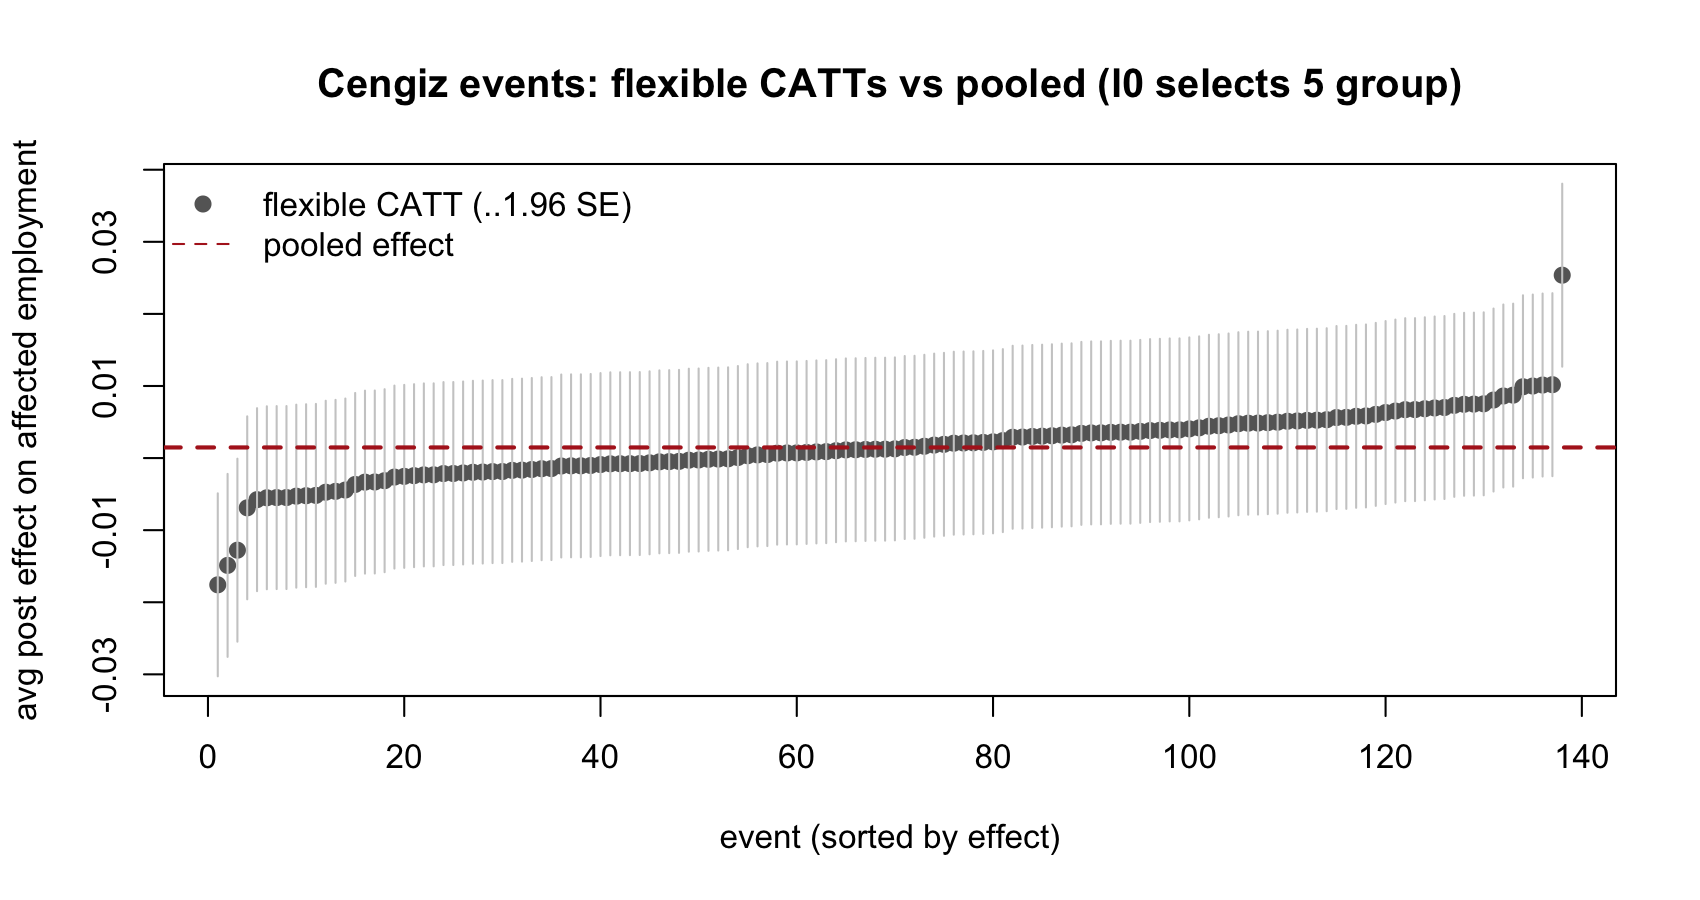
\includegraphics[width=0.8\linewidth]{cengiz_effects.png}
    \caption{The 138 event-level employment effects (average post-treatment coefficient on affected employment), sorted, with a common permutation-based confidence band; the dashed line is the pooled effect. The cross-event spread is no larger than the pre-trend noise band, and the pooled effect is near zero.}
    \label{fig:cengiz}
\end{figure}

Finally, we note that \citet{cengiz2019} themselves group events into three ``Card--Krueger'' bins defined ex ante by how binding the minimum wage is. Our exercise asks, and answers in the negative, a different question, whether the employment effects, taken as estimated, cluster into distinct levels. The two are complementary, in that grouping by a policy covariate is a modeling choice about expected heterogeneity, whereas our data-driven partition tests for realized heterogeneity in the effects and, here, finds none beyond noise.

\subsubsection{Diagnosing Canonical TWFE Bias: The Goodman-Bacon Decomposition}

To motivate the stacked design, we decompose the canonical (unstacked) two-way fixed effects estimand following \citet{goodman2021}. Two adjustments are needed to apply the decomposition here, since we proxy the affected workforce by employment below a fixed \$10 threshold (the true minimum-wage threshold moves across states and years), and we define treatment by the first increase a state enacts (to obtain an absorbing treatment). Both are conservative and, if anything, understate the bias.

Table~\ref{tab:bacon_decomp} reports the result. About $20\%$ of the estimand's weight comes from ``forbidden'' comparisons that use already-treated states as controls, and these carry a negative average estimate ($-0.006$), whereas the clean treated-versus-untreated comparisons (about $57\%$ of the weight) are positive ($0.006$). Because the pooled coefficient is the weighted average of these components, the already-treated controls bias it downward. This is the standard rationale for the stacked event-study design used above, and more broadly for taking the cohort-time effects, rather than a single pooled coefficient, as the objects of interest that the specification methods of this paper then group.

\begin{table}[H]
    \centering
    \caption{Goodman--Bacon decomposition of the canonical TWFE estimand (simplified absorbing-treatment panel).}
    \label{tab:bacon_decomp}
    \begin{tabular}{lcc}
        \toprule
        Comparison type & Weight & Average estimate \\
        \midrule
        Earlier vs.\ later treated & 0.236 & $\phantom{-}0.001$ \\
        Later vs.\ earlier treated & 0.195 & $-0.006$ \\
        Treated vs.\ untreated     & 0.569 & $\phantom{-}0.006$ \\
        \bottomrule
    \end{tabular}
\end{table}

% =============================================================================
% 7. CONCLUSION
% =============================================================================
\section{Conclusion}
\label{sec:conc}

This paper addresses a step in the staggered DiD workflow that has received
comparatively little attention, model specification. Once cohort-time effects are
identified as the estimands of interest, the researcher must still decide how many
distinct parameters to estimate. We frame this as a partition-selection problem
and address it with a Dirichlet Process mixture over the cohort-time effects. The
DP posterior assigns a probability to every grouping and reports full uncertainty,
including the uncertainty in the grouping itself, and is the object we recommend
for inference. Holding the error variance fixed, its maximum a posteriori
partition coincides with an $\ell_0$-penalized estimator, a connection to
the homogeneity-pursuit literature that we record as a remark rather than as a
separate recommendation. As a secondary benefit, the
partial-homogeneity restriction can also supply identifying information for a cell
that lacks a clean comparison, though that identification rests entirely on the
assumed grouping and is untestable for the cell that needs it.

The simulations and applications make the trade-offs concrete. Under partial
homogeneity with well-separated effect levels, both estimators cut the sampling
variance of the cohort-time effects by $26$--$52\%$ relative to the fully
flexible estimator at no bias cost, approaching the infeasible oracle as the
separation grows, with gains that vanish once the effects are nearly
indistinguishable, and the DP posterior
attains near-nominal coverage by marginalizing over the partition where naive
$\ell_0$-PH intervals are usable but mildly anti-conservative. The two
applications show both regimes on real data. In the minimum-wage and
teen-employment data of \citet{callaway2021} the effects are genuinely
heterogeneous and the method recovers a partially homogeneous structure,
collapsing seven effects into a few interpretable levels and roughly halving the
variance of the pooled cells while preserving the headline effect, whereas in the
low-wage-jobs study of \citet{cengiz2019} the $138$ event effects are
statistically indistinguishable from a common value and the method correctly
reports that pooling is adequate, functioning as a formal specification test. The
same procedure thus both exploits real heterogeneity and declines to manufacture
it where none exists.

Several directions merit future work. First, the agglomerative algorithm is a heuristic; developing exact or near-exact algorithms for small $K$, or theoretical guarantees on approximation quality, would be valuable. Second, honest inference after partition selection deserves a fuller theoretical treatment, since the naive $\ell_0$-PH intervals are conditional on the selected grouping (Remark~\ref{rem:postselection}), so developing valid selective-inference corrections for them (the Bayesian posterior already propagates partition uncertainty) is an open problem. Third, formal asymptotic theory establishing consistency of the partition estimator, as both $N$ and the effective sample size per CATT grow, would solidify the method's theoretical foundations, and would formalize the separation threshold that our simulations identify as the determinant of the efficiency gain. Finally, whereas covariate adjustment in the outcome equation is immediate (Section~\ref{sec:problem}, equations~\eqref{eq:twfe_cov}--\eqref{eq:resid_cov}), letting observable characteristics inform the grouping itself, through a covariate-dependent partition prior, is a more substantial extension that could improve performance in settings with richer data.

\appendix

\section{Identification under Limited Overlap}
\label{app:identification}

In some staggered designs a cohort-time cell lacks a clean comparison group, for
example when every unit is eventually treated and the last-treated cells have no
not-yet-treated or never-treated controls. Such a cell $k$ then contributes no
independent identifying variation, its within-transformed column $\tilde{D}_k$ is
collinear with the others, $\Dtd'\Dtd$ is singular, and the flexible estimator
$\hat{\tau}_{k,\text{flex}}$ is undefined for that coordinate. This is the
staggered-DiD counterpart of the lack-of-overlap problem in cross-sectional
designs, where the fully interacted (``long'') regression is not well defined
\citep{kwon2026}. Partial homogeneity offers a route through it, by letting the
unidentified cell inherit its group's effect. Let
$\mathcal{U} \subseteq \{1,\ldots,K\}$ be the set of cells not identified by the
flexible model and $\mathcal{U}^c$ its complement.

\begin{proposition}[Identification via partial homogeneity]
  \label{prop:identification}
  Suppose the true partition is $\mathcal{P} = \{C_1,\ldots,C_m\}$ and each group
  contains at least one identified cell, $C_p \cap \mathcal{U}^c \neq \emptyset$
  for every $p$. Then under the restricted model \eqref{eq:within} the group
  effect $\phi_p$ is identified for every $p$, and hence $\tau_k = \phi_p$ is
  identified for every $k \in C_p$, including the unidentified cells
  $k \in C_p \cap \mathcal{U}$.
\end{proposition}

\begin{proof}
Under $\mathcal{P}$ the group column is $\Dtd_p = \sum_{k\in C_p}\tilde{D}_k$, so
$\|\Dtd_p\|^2 \geq \sum_{k \in C_p \cap \mathcal{U}^c} n_k > 0$ whenever
$C_p \cap \mathcal{U}^c \neq \emptyset$. Under the orthogonal balanced-panel
design $\Dtd^{*\prime}\Dtd^*$ is then diagonal with strictly positive entries,
hence invertible, and each $\phi_p$ is estimable from \eqref{eq:oracle_var}.
Assigning $\tau_k = \phi_p$ identifies every cell in the group.
\end{proof}

Two caveats bound the result's practical reach. First, the identifying content
comes entirely from the restriction, not the data. An unidentified cell carries
no independent variation, so which group it belongs to cannot be learned from the
outcomes, and Proposition~\ref{prop:identification} is an identification result
conditional on the grouping whose recovered effect is only as credible as the
(untestable) assignment. Second, the argument is clean only in the orthogonal
case, where an unidentified cell is a zero column. Under general collinearity,
whether pooling restores identification depends on the partition in ways the
proposition does not settle. The Bayesian estimator's co-clustering probabilities
describe this assignment, but for a genuinely unidentified cell they are governed
by the prior rather than by evidence, so they should be read as prior belief
rather than as data.

\section{Computing the $\ell_0$-PH Estimator}
\label{app:algorithm}

The $\ell_0$-PH estimator is computed in two steps, an agglomerative search (a greedy sequence of pairwise merges) for the partition and an ordinary least squares re-estimation of the grouped model under it. This appendix gives both and shows why the re-estimation is necessary.

  \paragraph{Step 1: Partition recovery.} Exact minimization of $Q(\mathcal{P})$ over all partitions is NP-hard \citep{fan2001}; we solve it with
  an agglomerative algorithm that runs in $O(K^3)$ time, in the spirit of classical optimal-grouping procedures \citep{fisher1958}. Initialise with $K$ singleton groups, each assigned the flexible
  CATT estimate $\hat{\tau}_{k,\mathrm{flex}}$ and effective sample size $n_k = \|\tilde{D}_k\|^2$. At each iteration, compute
  for every pair of current groups $(A, B)$
  \begin{equation}
    \Delta\mathrm{Obj}(A, B) \;=\; \frac{n_A\, n_B}{n_A + n_B}\bigl(\hat{\tau}_A - \hat{\tau}_B\bigr)^2 \;-\; \lambda \cdot |A|
  \cdot |B|,
    \label{eq:deltaobj}
  \end{equation}
  where $n_A$, $n_B$ and $\hat{\tau}_A$, $\hat{\tau}_B$ are the current effective sample sizes and pooled estimates for groups
  $A$ and $B$ respectively. If $\min_{A \neq B}\,\Delta\mathrm{Obj}(A,B) \geq 0$, terminate and return the current partition
  $\hat{\mathcal{P}}$. Otherwise merge the minimizing pair, updating
  \begin{equation}
    \hat{\tau}_{A \cup B} \;=\; \frac{n_A\,\hat{\tau}_A + n_B\,\hat{\tau}_B}{n_A + n_B}, \qquad n_{A \cup B} \;=\; n_A + n_B.
    \label{eq:pooled}
  \end{equation}
  The algorithm terminates after at most $K - 1$ merges.

  \paragraph{Step 2: Re-estimation under the discovered partition.} Let $\hat{\mathcal{P}} = \{\hat{C}_1, \ldots,
  \hat{C}_{\hat{m}}\}$ denote the partition returned by Step~1. For each group $\hat{C}_p$, define the group regressor
  $\tilde{D}_p = \sum_{k \in \hat{C}_p} \tilde{D}_k$ and collect the $\hat{m}$ group regressors into the restricted
  within-transformed design matrix $\tilde{D}^* = [\tilde{D}_1, \ldots, \tilde{D}_{\hat{m}}]$. Estimate the restricted model
  \begin{equation}
    \tilde{Y} \;=\; \tilde{D}^*\phi + \tilde{\varepsilon}, \qquad \tilde{\varepsilon} \sim \bigl(0,\, \sigma^2 I_{NT}\bigr),
    \label{eq:step2}
  \end{equation}
  by OLS to obtain $\hat{\phi} = (\tilde{D}^{*\prime}\tilde{D}^*)^{-1}\tilde{D}^{*\prime}\tilde{Y}$. The $\ell_0$-PH CATT estimate
  for cell $k$ is $\hat{\tau}_k^{\ell_0} = \hat{\phi}_p$ for all $k \in \hat{C}_p$. Equivalently, \eqref{eq:step2} corresponds to
   the TWFE regression
  \begin{equation}
    Y_{igt} \;=\; \alpha_i + \gamma_t + \sum_{p=1}^{\hat{m}} \phi_p \sum_{k \in \hat{C}_p} D_{k,igt} + \varepsilon_{it},
    \label{eq:step2twfe}
  \end{equation}
  estimated on the full panel. We refer to the complete two-step procedure as the $\ell_0$-PH estimator.

  \paragraph{Why re-estimation is essential.} A natural one-step alternative uses the greedy-pooled values \eqref{eq:pooled}
  directly as CATT estimates. We show that this approach is generically inefficient and that the OLS re-estimation in Step~2 is a
   necessary correction, not a refinement.

  The greedy update $\hat{\tau}_{A \cup B}$ in \eqref{eq:pooled} is the weighted mean of the flexible estimates with weights $n_k
   = \|\tilde{D}_k\|^2$. Under the orthogonality condition $\tilde{D}_j'\tilde{D}_k = 0$ for $j \neq k$, which holds approximately in
  balanced panels in which each unit belongs to exactly one cohort, $\tilde{D}^{*\prime}\tilde{D}^*$ is diagonal with $p$-th
  diagonal entry $\|\tilde{D}_p\|^2 = \sum_{k \in \hat{C}_p} n_k$. In this case, the OLS estimate from Step~2 reduces to
  \begin{equation}
    \hat{\phi}_p \;=\; \frac{\tilde{D}_p'\tilde{Y}}{\|\tilde{D}_p\|^2} \;=\; \frac{\displaystyle\sum_{k \in \hat{C}_p}
  n_k\,\hat{\tau}_{k,\mathrm{flex}}}{\displaystyle\sum_{k \in \hat{C}_p} n_k},
    \label{eq:phorthog}
  \end{equation}
  which coincides with the greedy-pooled value \eqref{eq:pooled}. By Proposition~\ref{prop:oracle_dom}, $\hat{\phi}_p$ is therefore the BLUE of the
  group treatment effect, and Steps~1 and 2 deliver the same answer when the design is orthogonal.

  In general panels, however, cells belonging to the same treatment cohort share unit fixed effects, and cells falling on the
  same calendar period share time fixed effects. Both sources of co-occurrence produce non-zero off-diagonal elements in
  $\tilde{D}^{*\prime}\tilde{D}^*$, so the OLS estimate from Step~2,
  \begin{equation}
    \hat{\phi} \;=\; \bigl(\tilde{D}^{*\prime}\tilde{D}^*\bigr)^{-1}\tilde{D}^{*\prime}\tilde{Y},
    \label{eq:phgeneral}
  \end{equation}
  no longer reduces to the weighted mean \eqref{eq:pooled}. Three consequences follow. First, the greedy-pooled estimator does
  not satisfy the normal equations of \eqref{eq:step2} and therefore fails to be BLUE. Second, the $\Delta\mathrm{Obj}$ criterion
   \eqref{eq:deltaobj} is an approximation, in that it treats $\tilde{D}^{*\prime}\tilde{D}^*$ as diagonal when computing the RSS cost of
   each candidate merge, so partition selection in Step~1 rests on an approximate objective. Third, the greedy-pooled mean
  converges to $(n_A\tau_A^* + n_B\tau_B^*)/(n_A + n_B)$ rather than to the common group effect $\phi_p$ targeted by
  \eqref{eq:step2}, which undermines consistency whenever cells are not orthogonal.

  Step~2 corrects all three shortcomings simultaneously. Given any partition $\hat{\mathcal{P}}$, the estimator $\hat{\phi}$ in
  \eqref{eq:phgeneral} is the PH estimator of Proposition~\ref{prop:oracle_dom} applied to $\hat{\mathcal{P}}$. It is BLUE with variance
  $\sigma^2[(\tilde{D}^{*\prime}\tilde{D}^*)^{-1}]_{pp}$, which under orthogonality simplifies to $\sigma^2/\sum_{k \in
  \hat{C}_p} n_k$ and is strictly less than $\sigma^2/n_k$ for every $k \in \hat{C}_p$ whenever $|\hat{C}_p| \geq 2$, as
  established in \eqref{eq:var_ratio}. The efficiency gain is guaranteed by Gauss--Markov and grows with the size of the pooled
  group, and in the balanced case the variance ratio equals $n_k/\sum_{j \in \hat{C}_p} n_j < 1$, matching the ratio in
  \eqref{eq:var_ratio}. The one-step greedy-pooled estimator attains this gain only under exact orthogonality; Step~2 attains it
  unconditionally.

  The Bayesian estimator underscores the same point. Given a partition, its posterior mean of $\phi$ in \eqref{eq:bayes:phipost} solves the same grouped normal equations as \eqref{eq:step2} and, in the diffuse limit $\sigma_0^2 \to \infty$, equals $\hat{\phi}$ in \eqref{eq:phgeneral}. Both target the PH estimator under the discovered partition, whereas the one-step greedy-pooled mean does not.

\section{Heterogeneous Errors}
\label{app:hetero}

The model of Section~\ref{sec:bayes} assumes a scalar error variance, $\tilde\varepsilon \mid \tilde D \sim N(0,\sigma^2 I_{NT})$ in \eqref{eq:bayes:lik}. This appendix relaxes that assumption to a heterogeneous error covariance and records the few quantities that change, together with the augmented Gibbs sampler. Neither the partition prior \eqref{eq:bayes:partprior} nor the sampler's cluster-assignment logic is affected. The only changes are the design moments that enter the marginal likelihood and the group-effect posterior, and one additional Gibbs block that updates the variance parameters.

\paragraph{The modified model.} Replace the scalar covariance in \eqref{eq:bayes:lik} with a structured positive-definite matrix,
\begin{equation}
  \tilde\varepsilon \mid \tilde D \sim N(0,\Omega), \qquad \Omega = \bigoplus_{j=1}^{J}\sigma_j^2 I_{n_j},
  \label{eq:het:cov}
\end{equation}
where the $NT$ within-transformed observations are partitioned into $J$ variance blocks $\mathcal B_1,\dots,\mathcal B_J$ of sizes $n_1,\dots,n_J$, indexed by a known label $v(i)\in\{1,\dots,J\}$ for observation $i$. The blocks collect observations expected to share a noise level, for instance by cohort, by treated versus comparison status, or by an observed cluster. The homoskedastic model is the special case $J=1$. A fully general non-diagonal $\Omega$, such as the clustered influence-function covariance already used in the empirical applications (Remark~\ref{rem:sigma}), enters the formulas below in the same way through $\Omega^{-1}$, and only the update \eqref{eq:het:sigma} is specific to the block-diagonal parameterization. We complete the model with an independent conjugate prior on each variance level,
\begin{equation}
  \sigma_j^2 \sim \mathrm{Inv\text{-}Gamma}(a_0,b_0), \qquad j=1,\dots,J,
  \label{eq:het:prior}
\end{equation}
the natural generalization of \eqref{eq:bayes:sigma}.

\paragraph{What changes in the theory.} Every appearance of the precision $\sigma^{-2}I_{NT}$ becomes $\Omega^{-1}$. Writing the two design moments in the $\Omega^{-1}$ metric,
\begin{equation}
  S \;=\; \tilde D'\Omega^{-1}\tilde D, \qquad u \;=\; \tilde D'\Omega^{-1}\tilde Y,
  \label{eq:het:moments}
\end{equation}
the group effects still integrate out in closed form. Conditional on $\Omega$, the marginal likelihood \eqref{eq:bayes:marg} becomes $\tilde y\mid\mathcal P \sim N(\mu_0\tilde D\mathbf 1_m,\ \Omega+\sigma_0^2\tilde D\tilde D')$, and the Woodbury reduction \eqref{eq:bayes:logmarg}, dropping terms constant in $\mathcal P$, reads
\begin{equation}
  \log p(\tilde y\mid\mathcal P,\Omega) \;\propto\; -\tfrac12\log\bigl|\,I_m+\sigma_0^2 S\,\bigr| \;+\; \tfrac{\sigma_0^2}{2}\,u'\bigl(I_m+\sigma_0^2 S\bigr)^{-1}u.
  \label{eq:het:logmarg}
\end{equation}
The group-effect posterior \eqref{eq:bayes:phipost} becomes $\phi\mid\mathcal P,\Omega \sim N(\mu^*,\Sigma^*)$ with
\begin{equation}
  \Sigma^* \;=\; \bigl(S + I_m/\sigma_0^2\bigr)^{-1}, \qquad \mu^* \;=\; \Sigma^*\bigl(u + \mu_0\mathbf 1_m/\sigma_0^2\bigr),
  \label{eq:het:phipost}
\end{equation}
which is the ridge-regularized GLS estimator of the group effects. Setting $\Omega=\sigma^2 I_{NT}$ gives $S=\tilde D'\tilde D/\sigma^2$ and $u=\tilde D'\tilde Y/\sigma^2$ and recovers \eqref{eq:bayes:logmarg} and \eqref{eq:bayes:phipost} exactly. The computational cost is unchanged, the $m\times m$ matrix $S$ still governs the calculation, and forming it costs one weighting of the design by $\Omega^{-1}$, which is $O(NT)$ for the diagonal case \eqref{eq:het:cov}.

One feature of the fixed-$\sigma^2$ theory does not survive. The exact $\ell_0$ correspondence of Section~\ref{sec:freq}, in which the MAP partition minimizes the residual sum of squares plus a fixed penalty $L=\lambda\sigma^2$ per group, relied on the scalar variance factoring out of the objective. Under \eqref{eq:het:cov} the fit term is the $\Omega^{-1}$-weighted sum of squares and the variance levels also enter through $\log|\Omega|$, so the penalty is no longer a fixed multiple of a residual sum of squares. Heterogeneous errors are therefore handled inside the sampler, which averages over the variance levels along with the partition, rather than by the fixed-penalty point estimator.

\paragraph{The augmented Gibbs sampler.} The collapsed sampler of Section~\ref{sec:bayes:gibbs} gains one block. Given a current $\Omega$, one sweep runs the following three steps.
\begin{enumerate}
\item For each CATT $k$, remove $k$ from its cluster, delete the cluster if it is empty, and draw $z_k$ from the conditional probabilities \eqref{eq:bayes:condprob} with the marginal likelihoods now evaluated from \eqref{eq:het:logmarg}.
\item Draw the group effects $\phi \sim N(\mu^*,\Sigma^*)$ from \eqref{eq:het:phipost}.
\item Form the within-transformed residuals $\hat{\tilde\varepsilon} = \tilde Y - \tilde D_{\mathcal P}\phi$ under the current partition, and for each variance block draw
\begin{equation}
  \sigma_j^2 \mid \phi,\mathcal P,\tilde Y \;\sim\; \mathrm{Inv\text{-}Gamma}\!\Bigl(a_0+\tfrac{n_j}{2},\ b_0+\tfrac12\!\!\sum_{i\,:\,v(i)=j}\!\!\hat{\tilde\varepsilon}_i^{\,2}\Bigr),
  \label{eq:het:sigma}
\end{equation}
then assemble $\Omega=\bigoplus_j\sigma_j^2 I_{n_j}$ for the next sweep.
\end{enumerate}
Reinstating $\phi$ in Step~2 before the variance draw is what makes Step~3 conjugate, exactly as the original sampler reinstates $\phi$ to report the group effects. All posterior summaries of Section~\ref{sec:bayes:gibbs}, the CATT posterior mean \eqref{eq:bayes:tauhat}, the co-clustering matrix \eqref{eq:bayes:cocluster}, and the aggregated estimands, are formed from the augmented draws $\{z^{(s)},\phi^{(s)},\Omega^{(s)}\}$ without further change, so the reported credible intervals now propagate uncertainty in the error variances alongside the partition. When a plug-in covariance is preferred, fixing $\Omega$ at an estimate $\hat\Omega$ and omitting Step~3 recovers a single GLS-posterior sampler, the direct analog of the fixed-$\hat\sigma^2$ special case of Section~\ref{sec:bayes:sigmafixed}.

\section{Fixed versus Random $\sigma^{2}$}
\label{app:sigma}

The main text draws $\sigma^{2}$ from its inverse-gamma full conditional each sweep, the full Bayesian model of Section~\ref{sec:bayes:model}. Holding $\sigma^{2}$ fixed at the plug-in $\hat\sigma^{2}$ is the special case that yields the exact $\ell_0$ correspondence (Section~\ref{sec:bayes:sigmafixed}). This appendix shows the two give the same inference. We rerun the coverage experiment of Section~\ref{sec:sim:cov} at $m^{\ast}=6$ and $\delta=6$ over $500$ replications and, for each draw, form the DP credible intervals both ways from the same partition sampler.

\begin{table}[H]
  \centering
  \caption{Coverage and average length of nominal $95\%$ DP credible intervals
  under a random (full Bayesian) and a fixed (plug-in) error variance,
  $m^{\ast}=6$, $\delta=6$, $500$ replications.}
  \label{tab:sigma}
  \small
  \begin{tabular}{lcccc}
    \toprule
    & \multicolumn{2}{c}{CATT} & \multicolumn{2}{c}{ATT} \\
    \cmidrule(lr){2-3}\cmidrule(lr){4-5}
    $\sigma^{2}$ treatment & Coverage & Length & Coverage & Length \\
    \midrule
    Random (full Bayesian) & 0.94 & 0.20 & 0.95 & 0.11 \\
    Fixed (plug-in)        & 0.93 & 0.20 & 0.93 & 0.11 \\
    \bottomrule
  \end{tabular}
\end{table}

Table~\ref{tab:sigma} reports the result. The two samplers deliver essentially the same coverage and interval length, for the cohort-time effects and for the overall ATT. The reason is the one given in Section~\ref{sec:bayes:sigmafixed}, the residual degrees of freedom $NT - N - T + 1 - K$ are large, so $\sigma^{2}$ is pinned down and the estimation error a prior on it would propagate is negligible. The choice is therefore immaterial for the reported results, and we use the fixed-$\sigma^{2}$ case in the main text only to make the $\ell_0$ connection concrete.

% =============================================================================
% REFERENCES
% =============================================================================
\newpage
\bibliographystyle{aer}
\bibliography{references}

\end{document}
